\documentclass[twoside,english]{uiofysmaster}
\usepackage[utf8]{inputenc}
\usepackage[T1]{fontenc}
\usepackage[english]{babel}
\usepackage{epsfig}
\usepackage{graphicx}
\usepackage{caption}
\usepackage{subcaption}
\usepackage{amsfonts, amssymb, amsmath}
\usepackage{listings}
\usepackage{float}
\usepackage{hyperref}
\usepackage{epstopdf}
\usepackage{nomencl}
\makenomenclature

\usepackage[backend=bibtex]{biblatex}
% \bibliography{bibtex_ref_test.bib}
\bibliography{references.bib}

\renewcommand{\d}{\partial}
\renewcommand{\nomname}{List of Abbreviations}

\setlength{\headheight}{15pt}

% \usepackage{fontspec}
% \newfontfamily\listingsfont[Scale=0.85]{Droid Sans Mono}
% \lstset {
%     basicstyle=\footnotesize\listingsfont,
%     keywordstyle=\color{listingskeywordcolor}\footnotesize\listingsfont,
%     stringstyle=\color{listingsstringcolor}\footnotesize\listingsfont,
%     commentstyle=\color{listingscommentcolor}\footnotesize\listingsfont,
%     numberstyle=\gls{pde}\color{listingsnumbercolor}\footnotesize\listingsfont,
%     identifierstyle=\footnotesize\listingsfont,
% }



% compile with pdflatex --shell-escape main.tex
% makeindex main.nlo -s nomencl.ist -o main.nls

%opening
\author{Fredrik E Pettersen\\ f.e.pettersen@fys.uio.no}
\title{\uppercase{Multiscale modeling of diffusion processes in the brain}}
\date{June 2014}


\begin{document}


\maketitle

% \begin{abstract}
% This is an abstract text.
% \end{abstract}

% \begin{dedication}
%   To someone
%   \\\vspace{12pt}
%   This is a dedication to my cat.
% \end{dedication}

% \begin{acknowledgements}
%   I acknowledge my acknowledgements.
% \end{acknowledgements}


\tableofcontents
\clearpage
\listoffigures

\clearpage
\printnomenclature

% \clearpage
% \listoftables

\chapter{Introduction}
This thesis is an attempt at modeling diffusion processes in which part of the process takes place on a length scale so small that the continuum approximation becomes invalid. 
In this part we will therefore try and introduce another model of the diffusion process in the hope that this will give us something extra. 
It is the hope of Hans Petter that this thesis will be an introduction to a new research project to understand mesoscale physics in collaboration with Gaute Einevoll at UMB.

The very first approach was to simply try the problem on a bit. That is to try and substitute some small part of the mesh in a Finite Difference Diffusion solver (Froward Euler scheme) with a stochastic diffusion solver. A random walk method was implemented on part of the mesh to take over the equation-solving. This was done in 1 and 2 spatial dimensions with the aim of finding potential difficulties so that we can further investigate them. \\
Upon switching length-scales a fundamental question arises almost immediately; what is the continuum limit? In our case this question takes a slightly different, and possibly more answerable form; what is the conversion rate between the continuum model and the microscopic model, and by extension, what does a walker correspond to?
The first instinct of this candidate was to just try some conversion rate (say some value corresponds to some number of walkers), and this was implemented in both 1 and 2 dimensions.

\section{Background}
\emph{This is very much a first draft, and only my thoughts around what I understand as the basis of the thesis.}\\
Though the scope of this thesis might seem a bit \emph{sought}, it is in fact a real world concern from the computational neuroscience group at UMB. 
Their work contains network simulations of neurons, which they are trying to tweak with experimental data. 
The experimental data come from measurements of voltage levels in the Extra Cellular Space (ECS). 
The ECS is, essentially, the space which separates neurons and has an immensely complicated geometry as we can see from figure \ref{ECS_picture}. 
The width of the ECS varies, but is in general $\sim1\mu$m. 
Parts of the ECS is, however, much narrower. In the ECS there are a number of diffusion governed transport mechanisms which are vital for the function of the neurons. 
In fact, there are examples of snake venom which have a shrinking effect on the ECS, and it is thought that this causes large scale neuronal death very quickly. 
For the researchers at UMB, however, the ECS is of importance because the diffusion tensor in the ECS is related to the conductivity tensor through equation \ref{conductivity_diffusion_eq}, which in turn lets them teak parameters in their network models. \\
\begin{equation}\label{einstein_viscosity}
D = \frac{k_B T}{6\pi \eta r},
\end{equation}
Though there are several reasons to study diffusion processes in the ECS, this project has a specific goal in mind. 
The Einstein relation, eq. (\ref{einstein_viscosity}), relates the diffusion constant to the viscosity of the medium in which the diffusion is taking place. 
From the definition of viscosity, $\mu$, we have 
\begin{equation}
v_d = \mu F 
\end{equation}
where $F = qE$ is the standard electrical force acting on a charged particle. 
We can also define the current from the drift velocity of the particles as 
\begin{equation}
J = cqv_d = \sigma E 
\end{equation}
where $\sigma = c\mu q^2$ is the electrical conductance, in this case, of the ECS. 
Inserting this in the Einstein relation, eq. (\ref{einstein_viscosity}), lets us express the conductivity in terms of the diffusion constant as 
\begin{equation}\label{conductivity_diffusion_eq}
\sigma = \frac{cq}{k_B T}D 
\end{equation}
Equation (\ref{conductivity_diffusion_eq}) is trivially generalizable to tensor notation, where the conductance and diffusion ``constant'' are both 2. order tensors.\\

\begin{equation}\label{stochastic_einstein}
\langle r^2\rangle = 2dDt 
\end{equation}

The fundamental problem here is that, while diffusion in its own is a truly multi-scale process, we have no way of knowing for sure that the continuum models, and all they bring with them, are correct for this type of geometry. 
In particular, the Einstein relation \ref{einstein_viscosity} has, to my knowledge, only been derived for diffusion in a homogeneous media. 
The definition of a homogeneous media includes a mean free path close to infinity, which we will have trouble arguing for the existence of in the ECS. 
On the other hand, I know that another Einstein relation \ref{stochastic_einstein} is widely used  in other fields of physics where the media in question is hardly homogeneous. 
In molecular dynamics simulations, the two mentioned Einstein relations are used to measure the viscosity of fluids in nano-porous materials, and with success as far as I know.

\section{A short introduction to mathematical neuroscience}

Neuroscience is the scientific study of the nervous system, but in the traditional sense it focuses very much on what parts of the brain are responsible for what. 
Mathematical neruroscience is more focused on the physics and chemistry involved in the different parts of the brain and nervous system. 
An example of the power of this approach is the classical work done by Hodgkin and Huxley in 1952, earning them the Nobel price in Physiology or medicine in 1963. 
Through four non-linear coupled differential equations they were able to predict the propagation speed of signals along the squid giant axon to a quite high precision. \\

% Copied from the project

The human brain consists of two types of cells; the neurons and neuroglia. 
Neurons are tasked with signal processing and transport, while the glia are thought to have more janitorial tasks. 
The neurons are bathed in a salt solution that is mainly $Na^+$ and $Cl^-$. 
Inside the neurons, a highly regulated salt solution of mainly $K^+$ sets up a potential difference relative to the outside of the cell of approximately $-65$mV.
The neurons are in constant communication with each other through action potentials, which are disturbances in the membrane potentials of neurons. 
These action potentials are generated in the body of the cell, called the soma, from where they propagate down the axon without loss of amplitude. 
This is achieved by constantly amplifying the signal using ion pumps (see the Hodgin-Huxley model of the action potential \cite{sterratt2011principles}).
After propagating down the axon, the action potential reaches a synapse which is a gate to another neuron. 
If the action potential is of significant strength, vesicles carrying neurotransmitters merge with the synapse membrane, letting the neurotransmitters diffuse to the dendrite of the other neuron. 
If enough neurotransmitters reach the post-synaptic side, the signal continues propagating to the soma of this neuron, and the entire process starts over again. \\
The interest of this project lies, mainly, in the diffusion processes that take place in the space between these types of cells, the so-called extracellular space (ECS). 
This is a narrow space ($\sim 10-100$ nm \cite{nicholson2001diffusion}) with a highly complicated geometry (Figure \ref{ECS}). 
Surprisingly, the ECS adds up to $20\%$ of the total brain volume. 
We can understand this by realizing that every part of a cell must be separated from another cell by the ECS. 
Since the cells consists of axons and dendrites which can be viewed as (somewhat) fractal, we see that this means separating a vast amount of surface area from other surface areas.

The ECS is thought to support the diffusion of oxygen and nutrients to the neurons and glia, and diffusion of carbon dioxide and other waste from these cells through the blood - brain barrier and into the bloodflow. 

% \section{Dendritic spines}




\chapter{Basic Theory}

In this chapter we will take a closer look at random walks, both in general and the transition from the statistical view to partial differential equations. 
We will take a look at different algorithms to produce random walks, and discuss their pros and cons in light of this project. 
Then we will take a quick look at partial differential equations and numerical solution of them.

\section{Introduction to random walks}\label{introduction_to_random_walks}
The most basic random walk is a walker on the x-axis which will take a step of a fixed length to the right with a probability $p$, or to the left with a probability $q=1-p$. 
Using (pseudo-) random numbers on a computer we can simulate the outcomes of a random walk. 
For each step (of which there are N) we draw a random number, r, between 0 and 1 from some distribution (say a uniform one) which will be the probability. 
If $r\leq p$ the walker will take a step to the left, otherwise it will take a step to the right. 
After the N steps the walker will have taken R steps to the right, and $L = N-R$ steps to the left. 
The net displacement from the origin will be $S = R-L$. \\
This simple approach is easily generalizable to two and three dimensions by having $2d$ possible outcomes from the random number, where d is the dimensionality. 
In two dimensions the walker will step up if $r\in(0.75,1]$ and left if $r\in[0,0.25)$, for example.

\subsection{Further discussion and analysis of the introduction}\label{further_introduction}
The following derivation is borrowed from a compendium in statistical mechanics by Finn Ravndal. \\
If we do sufficiently many walks, the net displacement will vary from $S=+N$ to $S=-N$ representing all steps to the right and all steps to the left respectively. 
The probability of all steps being to the right is $P_N(N) = p^N$. 
Should one of the steps be to the left, and the rest to the right we will get a net displacement of $S = N-2$ with the probability $P_N(R = N-1) = Np^{N-1}q$. 
We can generalize this to finding the probability of a walk with a R steps to the right as 
\begin{equation}\label{bernoulli_distr}
 P_N(R) = {N\choose R}p^{R}q^{N-R}
\end{equation}
where ${N\choose R}=\frac{N!}{R!(N-R)!}$ is the number of walks which satisfy the net displacement in question, or the multiplicity of this walk in statistical mechanics terms. 
Equation \ref{bernoulli_distr} is the Bernoulli probability distribution, which is normalized.
\begin{align*}
 \sum\limits_{R=0}^N P_N(R) = (p+q)^N = 1^N = 1
\end{align*}
We can use this distribution to calculate various average properties of a walk consisting of N steps. 
For example, the average number of steps to the right is
\begin{align*}
 \langle R\rangle &=  \sum\limits_{R=0}^N RP_N(R) =  \sum\limits_{R=0}^N {N\choose R}Rp^Rq^{N-R} = \\
 p\frac{d}{dp} \sum\limits_{R=0}^N {N\choose R}p^Rq^{N-R} &= p\frac{d}{dp}(p+q)^N = Np(p+q)^{N-1} = Np
\end{align*}
From this we can also find the average value of the net displacement using $S = R-L = R-(N-R) = 2R-N$.
\begin{align*}
 \langle S\rangle = \langle2R\rangle -N = 2Np-N(p+q) = N(2p-p-q) = N(p-q)
\end{align*}
We notice that the average net displacement is greatly dependent on the relationship between $p$ and $q$, and that any symmetric walk will have an expected net displacement of zero. 
In many cases we will be more interested in the mean square displacement than the displacement itself, because many important large scale parameters can be related to the root-mean-square displacement. 
This can also be calculated rather straightforwardly. 
\begin{align*}
  \langle R^2\rangle =  \sum\limits_{R=0}^N R^2P_N(R) &=  \sum\limits_{R=0}^N {N\choose R}R^2p^Rq^{N-R} = \\
 \left(p\frac{d}{dp}\right)^2 \sum\limits_{R=0}^N {N\choose R}p^Rq^{N-R} &= \left(p\frac{d}{dp}\right)^2(p+q)^N \\
 = Np(p+q)^{N-1} +p^2N(N-1)(p+q)^{N-2} &= (Np)^2 +Np(1-p) = (Np)^2 +Npq
\end{align*}
Like before, the average net displacement is given as $S^2 = (2R-N)^2$ and we obtain
\begin{align*}
 \langle S^2\rangle = 4\langle R^2\rangle -4N\langle R\rangle + N^2 &= 4((Np)^2 +Npq) -4N^2p + N^2\\
 = N^2(4p^2 -4p +1) +4Npq &= N^2(2p-1)^2 +4Npq = N^2(p-q)^2 +4Npq.
\end{align*}
which for the 1D symmetric walk gives $\langle S^2\rangle =N$ and the variance, denoted $\langle\Delta S^2\rangle = \langle\langle S^2\rangle-\langle S\rangle^2\rangle$, is found by insertion as
\begin{align}
 \langle\Delta S^2\rangle &= \langle N^2(p-q)^2 +4Npq - ( N(p-q))^2\rangle= 4Npq 
\end{align}

When the number of steps gets very large we can approximate the Bernoulli distribution (eq. \ref{bernoulli_distr}) by the Gaussian distribution. 
This is most easily done in the symmetric case where $p=q=\frac{1}{2}$, but it is sufficient for the steplengths to have a finite variance (\emph{find something to refer to}). 
The Bernoulli distribution then simplifies to
\begin{equation}
 P(S,N) = \left(\frac{1}{2}\right)^N\frac{N!}{R!L!}
\end{equation}
on which we apply Stirling's famous formula for large factorials $n!\simeq\sqrt{2\pi n}\cdot n^ne^{-n}$.
\begin{align*}
 P(S,N) &= \left(\frac{1}{2}\right)^N\frac{N!}{R!L!} \\
 &= \exp\left(-N\ln2+\ln\sqrt{2\pi N}+N\ln N - \ln\sqrt{2\pi R} -R\ln R - \ln\sqrt{2\pi L} - L\ln L \right) \\
 &= \sqrt{\frac{N}{2\pi RL}}\exp\left(-R\ln\frac{2R}{N}-L\ln\frac{2L}{N}\right)
\end{align*}
Where we have used $R+L=N$. We now insert for $\frac{2R}{N}=1+\frac{S}{N}$ and $\frac{2L}{N}=1-\frac{S}{N}$ and expand the logarithms to first order, $RL=\frac{N^2-S^2}{4}$ in the prefactor, and approximate $1-\frac{S^2}{N^2}\simeq1$. This gives
\begin{equation}\label{descrete_gaussian_distr}
 P(S,N) =\sqrt{\frac{2}{\pi N}}\exp\left(\frac{-S^2}{2N}\right)
\end{equation}
which is an ordinary, discrete Gaussian distribution with $\langle S\rangle = 0$  and $\langle S^2\rangle = N$. 
If we keep assuming that the walker is on the x-axis, and let the step length, a, get small the final position will be $x=Sa$ which we can assume is a continuous variable. 
Similarly, we let the time interval between each step, $\tau$, be small and let the walk run for a continuous time $t=N\tau$. This changes the distribution \ref{descrete_gaussian_distr} to
\begin{equation}
 P(x,t) = \frac{1}{2a}\sqrt{\frac{2\tau}{\pi t}}\exp\left(-\frac{x^2\tau}{2a^2t}\right). 
\end{equation}
The prefactor $\frac{1}{2a}$ is needed to normalize the continuous probability distribution since the separation between each possible final position in walks with the same number of steps is $\Delta x=2a$. 
We also introduce the diffusion constant
\begin{equation}
D = \frac{a^2}{2\tau} 
\end{equation}
making the distribution
\begin{equation}
 P(x,t) = \sqrt{\frac{1}{4\pi Dt}}\exp\left(-\frac{x^2}{4Dt}\right)
\end{equation}

Introducing $x$ also gives us the expectation value and variance of x on a form which will be useful later. 

We have $x=Sa$ which means 
$$\langle x\rangle=a\langle S\rangle$$ 
and 
$$\langle x^2\rangle=a^2\langle S^2\rangle$$
Finally by insertion we find the variance $\langle \Delta x^2\rangle$
\begin{equation}\label{random_walk_variance}
 \langle \Delta x^2\rangle = \langle\langle x^2\rangle -\langle x\rangle^2\rangle = \langle a^2\langle S^2\rangle -a^2\langle S\rangle^2\rangle = 4Npqa^2
\end{equation}


\subsection{More general Random Walks}\label{more_general_random_walks}

In the more general case, the position of a random walker, $\vec{r}$ at a time $t_i$ is given by the sum
\begin{equation}\label{brownian_motion}
 \vec{r}(t_i)=\sum\limits_{j=0}^i \Delta \vec{x}(t_j)
\end{equation}
where $\Delta \vec{x}(t_j) = \left(\Delta x(t_j),\Delta y(t_j),\Delta z(t_j)\right)$ in 3D. Each $\Delta x,\Delta y,\Delta z$ is a random number drawn from a distribution with a finite variance $\sigma^2 = \langle\Delta x^2\rangle$. 
By the central limit theorem, any stochastic process with a well defined mean and variance can, given enough samples, be approximated by a Gaussian distribution. 
This means that the probability of finding the walker at some position x after M steps is 
\begin{equation}
 P(x,M)\propto e^{-\frac{x^2}{2M\sigma^2}}
\end{equation}
Remember that the actual Gaussian distribution is 
$$
\frac{1}{\sqrt{2\pi\sigma^2}}\exp\left(\frac{(n-\mu)^2}{2\sigma^2}\right)
$$

We can introduce an Einstein relation $\sigma^2 = 2dD\Delta t$ and the obvious relation $t = M\Delta t$ to get a more desirable exponent.
We see that $\langle \Delta x^2\rangle = 2Dt$ in the one dimensional case where $d=1$. 

\emph{The introduction of the Einstein relation might put some restrictions on our model.}
Normalizing the expression gives us 
\begin{equation}\label{rw_gaussian_distribution}
 P(x,t) = \sqrt{\frac{1}{4Dt}}\exp\left(-\frac{x^2}{4Dt}\right)
\end{equation}

If we have a large number, N, of walkers, their concentration will be $C(x,t) = NP(x,t)$. 
The concentration is conserved, so any amount that flows out of an area must reflect as a decrease in concentration. 
We can express this by the flow of concentration
\begin{equation}
 \frac{\d C}{\d t} -\nabla\cdot\vec{J} = S
\end{equation}
where $\vec{J}$ is the flow vector and S is a source term which in our case will be zero.
From Fick's first law we know that $\vec{J} = -D\nabla C$. Inserting this gives us
\begin{equation}\label{simple_diffusion_equation}
 \frac{\d C}{\d t} = \nabla\cdot \left(D\cdot\nabla C\right)
\end{equation}
which is the diffusion equation.
By insertion we can check that this version (\ref{rw_gaussian_distribution}) of the Gaussian distribution fulfills the diffusion equation. 
Starting with only the time derivative gives us
\begin{align*}
 \frac{\d P}{\d t} = -\frac{4\pi D\exp\left(-\frac{x^2}{4Dt}\right)}{2\sqrt{(4\pi Dt)^3}}&+\frac{x^2\exp\left(-\frac{x^2}{4Dt}\right)}{4Dt^2\sqrt{4\pi Dt}} \\
 = \exp\left(-\frac{x^2}{4Dt}\right)\left(\frac{8Dx^2}{2\sqrt{\pi}(4Dt)^{5/2}} -\frac{(4D)^2t}{2\sqrt{\pi}(4Dt)^{5/2}}\right)&= \frac{4D\exp\left(-\frac{x^2}{4Dt}\right)(x^2-2Dt)}{\sqrt{\pi}(4Dt)^{5/2}}
\end{align*}
 We then finish by doing the spatial derivative
\begin{align*}
 D\frac{\d^2 P}{\d x^2} &= \frac{D}{\sqrt{4\pi Dt}}\frac{\d}{\d x}\left[-\exp\left(\frac{-x^2}{4Dt}\right)\left(\frac{-2x}{4Dt}\right)\right]\\
 = \frac{2D}{4Dt\sqrt{4\pi Dt}}&\exp\left(\frac{-x^2}{4Dt}\right)\left[1-x\left(\frac{2x}{4Dt}\right)\right] = \frac{4D\exp\left(-\frac{x^2}{4Dt}\right)(x^2-2Dt)}{\sqrt{\pi}(4Dt)^{5/2}}
\end{align*}
and see that they are equal, meaning that the diffusion equation is satisfied.

\subsection{Choosing random walk algorithm}\label{choosing_random_walk_algorithm}

The simplest random walk model, which places walkers on discrete mesh points and uses a fixed step length, has been used with great success to model diffusion processes. 
Farnell and Gibson discuss this in their article \cite{farnell2005monte}. 
In this project we will be torn between chosing a realistic algorithm to advance the random walkers, like brownian motion or to go for simplicity. 
That being said, by the central limit theorem both models will after some timesteps be described by a Gaussian distribution meaning that on the PDE scale we will not know the difference. 
Hence it will make no sense to not use the simplest random walk model.
We should note that it will be quite easy to change the algorithm used for random walks, and so we have not locked ourselves to anything yet.

\subsection{Random walks and anisotropy}\label{random_walks_and_anisotropy}

Any real problem where parts of the diffusion process cannot be modelled by the continuum approximation is bound to be anisotropic. 
There is reason to believe that an anisotropic diffusion process on the PDE level will lead to an anisotropic random walk model as well, but how do we model this. 
If we simply replace the diffusion constant by a function $D = D(\vec{x})$ (see eq \ref{steplength}) we are at least started, but this will not quite be sufficient as Farnell and Gibson point out \cite{farnell2005monte}. 
Through their experiments they found that only adjusting the steplength will not improve the error noticeably and reasoned that this is because the walkers are still as likely to jump in both directions (right or left in 1d), and that the stepsize is the same in both cases, hence the model does not resemble anisotropy. 
They went on to introduce an adjusted steplength and an adjusted step probability, a solution they landed on after trial and error. 
The expressions they proposed are listed in equations \ref{farnell_and_gibson_1} to \ref{farnell_and_gibson_5}. 
\begin{equation}\label{farnell_and_gibson_1}
 \Delta_p(x) = \frac{1}{2}\left(L(x) + L(x +\Delta_p(x))\right) \to L(x) +\frac{1}{2}L(x)L'(x)
\end{equation}
\begin{equation}\label{farnell_and_gibson_2}
 \Delta_m(x) = \frac{1}{2}\left(L(x) + L(x -\Delta_m(x))\right) \to L(x) +\frac{1}{2}L(x)L'(x)
\end{equation}
where $L(x)$ is defined in equation \ref{farnell_and_gibson_3} and $\Delta_p(x)$ and $\Delta_m(x)$ are the adjusted steplengths to the right and left, respectively.
\begin{equation}\label{farnell_and_gibson_3}
L(x) = \sqrt{2D(x)\Delta t}
\end{equation}
We also have the adjusted jump probabilities $T_r(x)$ and $T_l(x)$ which are the probabilities for a walker at position x to jump right or left, respectively. 
These are defined in equations \ref{farnell_and_gibson_4} and \ref{farnell_and_gibson_5}
\begin{equation}\label{farnell_and_gibson_4}
T_r(x) = \frac{1}{2} +\frac{1}{4}L'(x)
\end{equation}
\begin{equation}\label{farnell_and_gibson_5}
T_l(x) = \frac{1}{2} -\frac{1}{4}L'(x)
\end{equation}
We notice that the adjusted steplength we proposed to start with is still a part of the final expressions.


\subsection{Random walks and drift}\label{random_walks_and_drift}

Another point we have yet to say something about is diffusion that has a drift term, $\frac{\d u}{\d x}$. 

Initially one thought that diffusion in the Extra Cellular Space of the brain was governed by a drift term, but the modern perception is that this drift term is in the very least negligible \cite{nicholson2001diffusion}. 
Though it is unlikely that we will include a drift term in our model, we will say a few words about it here since it is of importance in other applications and might be a natural extension at some point, should someone else use this work.\\
We model random walkers with drift by simply adding some vector to the Brownian motion model, thus forcing all walkers to have a tendency to walk a certain direction. 
This approach can also be used in the fixed steplength (or variable steplength in the anisotropic case)  if we express the new step, $\vec{s}$, as
\begin{align*}
 \vec{s} = (\pm l \text{ or }0,\pm l \text{ or }0) +\vec{d}
\end{align*}
where $\vec{d}$ denotes the drift of the walker.\\
We can set up the continuity equation for a concentration, $C(x,t) = NP(x,t)$ of random walkers which are affected by a drift.
\begin{equation}
 \frac{\d C}{\d t} +\nabla\cdot\vec{j} = S
\end{equation}
Where $\vec{j}$ denotes the total flux of walkers through some enclosed volume and $S$ is a source/sink term. 
Since the walkers are affected by drift the flux will consist of two terms; $\vec{j} = \vec{j}_{diff}+\vec{j}_{drift}$. 
From Fick's first law we know that $\vec{j}_{diff} = -D\nabla C$. 
The second flux term is the advective flux which will be equal to the average velocity of the system; $\vec{j}_{drift} = \vec{v}C$. 
Inserting this in the continuity equation gives us the well known convection diffusion equation (\ref{convection_diffusion_equation}).
\begin{equation}\label{convection_diffusion_equation}
 \frac{\d C}{\d t} = \nabla\cdot\left(D\nabla C\right)-\nabla\cdot\left(\vec{v}C\right) + S
\end{equation}
Which in many cases will simplify to
\begin{equation}
 \frac{\d C}{\d t} = D\nabla^2 C-\vec{v}\cdot\nabla C
\end{equation}

In order to determine all the parameters of the convection diffusion equation \ref{convection_diffusion_equation} we will need to go through some of the calculations from chapter \ref{introduction_to_random_walks}. 
The situation is the same, a walker in one dimension which can jump left or right, but this time will also move a finite distance $d$ each timestep. 
This will make the expected net displacement
\begin{equation*}
 \langle S\rangle = R-L +Nd = N(p-q) + Nd
\end{equation*}
and the expected mean square displacement
\begin{equation*}
 \langle S^2\rangle = (2\langle R\rangle -N)^2 +(Nd)^2 = N^2(p-q)^2 +4Npq +(Nd)^2
\end{equation*}
which in turn gives us the variance
\begin{align*}
 \langle \Delta S^2\rangle &= \langle\langle S^2\rangle-\langle S\rangle^2\rangle \\
 &= N^2(p-q)^2 +4Npq +(Nd)^2 - N^2(p-q)^2 -(Nd)^2 \\
\langle \Delta S^2\rangle &= 4Npq
\end{align*}
This shows us that the variance is untouched by the drift term, but not the mean which for the symmetric case is $\langle S\rangle = Nd$. 
When we convert this to the continuous variables $x$ and $t$ we get the solution shown in equation \ref{solution_convection_diffusion_eq}.
\begin{equation}\label{solution_convection_diffusion_eq}
 C(x,t) = \frac{N}{\sqrt{4\pi Dt}}\exp\left(-\frac{(x-vt)^2}{4Dt}\right)
\end{equation}
Where $v = \frac{d}{\Delta t}$ is the velocity of the concentration and $D$ is the well known diffusion constant, inserted from the Einstein relation $\sigma^2 = 2D\Delta t$.\\

%%%%%% Not sure if this should be included %%%%%%%%%

% The only problem with the solution \ref{solution_convection_diffusion_eq} is that it is invalid for $t=0$. 
% In order to use it we will need an initial condition which fits the rest of the solution. 
% We try and find this by first checking by simulation if it converges towards some initial solution as $t\to0$ and if so, extrapolate this to $t=0$ as the initial condition. 
% Figure \ref{convection_diffusion_eq_initial_condition} shows the result of this little experiment, and as we clearly see it does diverge as $t\to0$. 
% However, it also converges to a Dirac delta function, $\delta(x)$ which is defined by its properties
% \begin{align*}
% \delta(x) = \begin{cases} +\infty, & x = 0 \\ 0, & x \ne 0 \end{cases}
% \end{align*}
% and
% \begin{equation*}
%  \int_{-\infty}^\infty \delta(x) \, dx = 1
% \end{equation*}
% The Dirac delta function often sought as an initial condition in experimental setups for measurements on diffusion processes because of its compatibility with a variety of diffusion equations, and should do a very good job in our numerical setup as well. 
% 
% \begin{figure}[H]
%  \centering
%  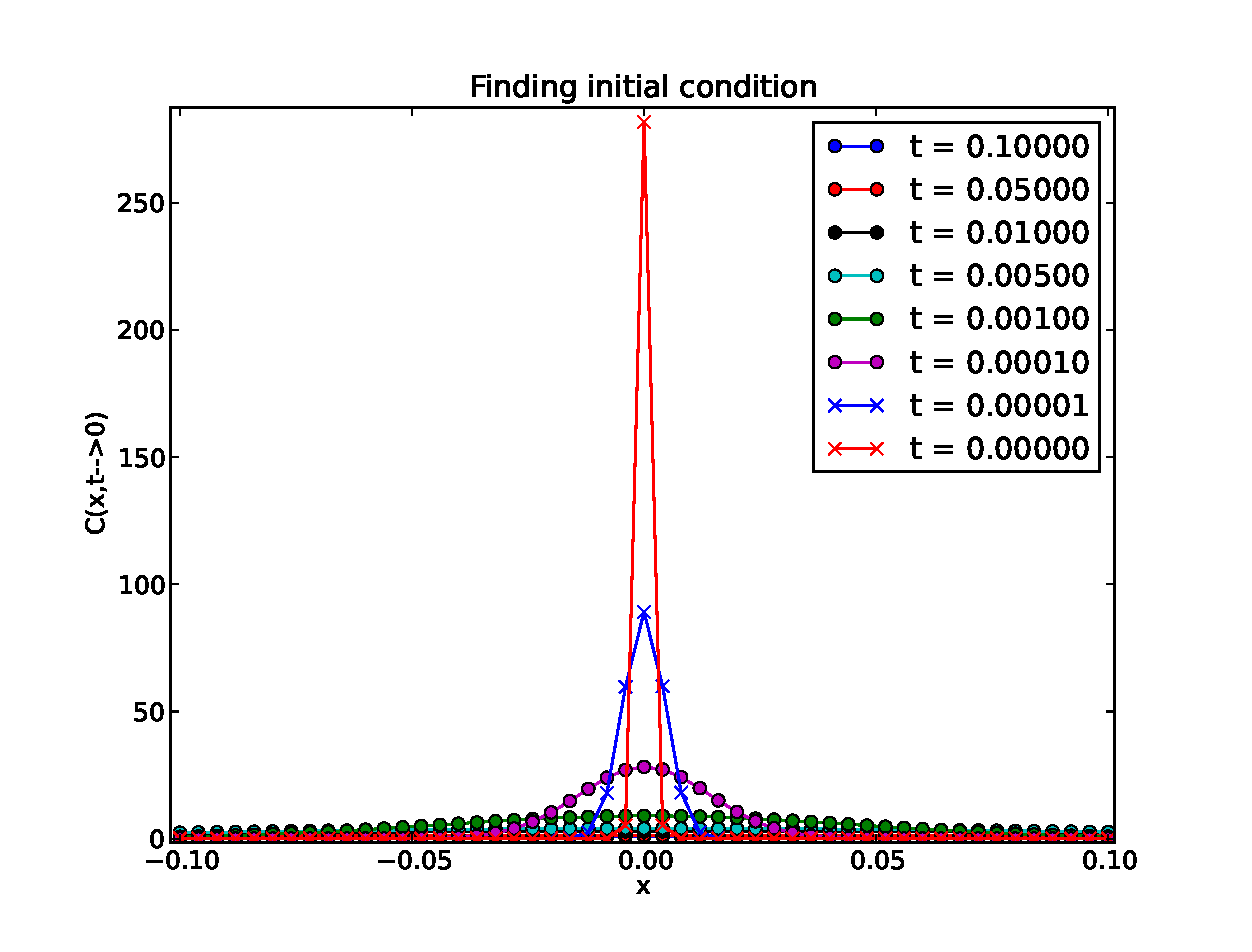
\includegraphics[scale=0.7]{Figures/convection_diffusion_eq_initial_condition.eps}
%  \caption[Initial condition for convection diffusion]{Experiment to determine the initial condition of equation \ref{solution_convection_diffusion_eq}}
%  \label{convection_diffusion_eq_initial_condition}
% \end{figure}


\section{Some words about partial differential equations}\label{some_words_on_PDEs}
\subsection{Discretizing}\label{discretizing}

To maintain a bit of generality we will look at the (potentially) anisotropic diffusion equation in 2d. The extension to 3d is trivial, as is the 1d version.
\begin{equation}
 \frac{\d u}{\d t} = \nabla D\nabla u +f
\end{equation}
where f is some source term. 
The final expression and scheme will depend on how we chose to approximate the time derivative, but the spatial derivative will have the same approximation. \\
We start off by doing the innermost derivative in one dimension. 
The generalization to more dimensions is trivial, and will consist of adding the same terms for the y and z derivatives. 
\begin{align*}
 \left[\frac{d}{dx}u\right]^n \approx \frac{u^n_{i+1/2}-u^n_{i-1/2}}{\Delta x}
\end{align*}
Where we have made the approximate derivative around the point $x_i$. 
We then set $\phi(x)=D\frac{du}{dx}$ and do the second derivative
\begin{align*}
  \left[\frac{d}{dx}\phi\right]^n \approx \frac{\phi^n_{i+1/2}-\phi^n_{i-1/2}}{\Delta x}
\end{align*}
and insert for $\phi$
\begin{align*}
 \frac{\phi^n_{i+1/2}-\phi^n_{i-1/2}}{\Delta x} = \frac{1}{\Delta x^2}\left(D_{i+1/2}(u^n_{i+1}-u^n_{i+1}) -D_{i-1/2}(u^n_{i}-u^n_{i-1})\right)
\end{align*}
Since we can only evaluate the diffusion constant at the mesh points (or strictly speaking since it is a lot simpler to do so) we must approximate $D_{i\pm1/2}\approx0.5(D_{i\pm1}+D_i)$. 
Inserting this gives us 
\begin{align*}
 \nabla D\nabla u\approx\frac{1}{2\Delta x^2}\left((D_{i+1,j}+D_{i,j})(u_{i+1,j}-u_{i,j})-(D_{i,j}+D_{i-1,j})(u_{i,j}-u_{i-1,j})\right) \\
 +\frac{1}{2\Delta y^2}\left((D_{i,j+1}+D_{i,j})(u_{i,j+1}-u_{i,j})-(D_{i,j}+D_{i,j-1})(u_{i,j}-u_{i,j-1})\right)
\end{align*}

The discretization of the time-derivative is where we can see a difference between the two schemes we will use in this project. 
When ordinary differential equations are discretized one can clearly see how this difference arises, and so we will write our PDE \nomenclature{PDE}{Parital Differential Equation} using a new notation
\begin{equation}
 D_t u = Ou
\end{equation}
where the right-hand-side operator $O$ indicates some operation like the double spatial derivative. 
Introducing the general discretization of the time derivative gives us equation \ref{theta_rule} known as theta-rule. 
Setting $\theta = 0$ yields the FE\nomenclature{FE}{Forward Euler} discretization, and $\theta = 1$ the BE \nomenclature{BE}{Backward Euler} discretization. 

\begin{equation}\label{theta_rule}
 \frac{u^{n+1}-u^n}{\Delta t} = O\left(\theta u^{n+1} +(1-\theta)u^n\right)
\end{equation}

From the theta rule we can see that the only difference between the FE and BE scheme is at what time-step we evaluate the right-hand-side of the equation. 
The theta-rule can give other schemes as well, using some weighted average of the right-hand-side at $t^n$ and $t^{n+1}$ but we will not look into these in this project. 
We can now summarize by writing out the FE discretization as it will be implemented in 1d in equation \ref{FE_scheme_1D}.

\begin{align}\label{FE_scheme_1D}
 u^{n+1}_i = \frac{\Delta t}{2\Delta x^2}\left((D_{i+1}+D_{i})(u^n_{i+1}-u^n_{i})-(D_{i}+D_{i-1})(u^n_{i}-u^n_{i-1})\right) + u^n_i
\end{align}

We will come back to the FE discretization when we discuss stability later. \\
Looking at the BE discretization which is written out in 1d in equation \ref{BE_scheme_1D} we notice that there are quite a few more unknowns per mesh-point. 

\begin{align}\label{BE_scheme_1D}
 u^{n+1}_i = \frac{\Delta t}{2\Delta x^2}\left((D_{i+1}+D_{i})(u^{n+1}_{i+1}-u^{n+1}_{i})-(D_{i}+D_{i-1})(u^{n+1}_{i}-u^{n+1}_{i-1})\right) + u^n_i
\end{align}

Writing out the calculations for a small mesh we recognize a pattern which we can exploit.
\begin{align*}
 &u^{n+1}_0 =  \frac{\Delta t}{2\Delta x^2}\left(2(D_{0}+D_{1})(u^{n+1}_{1}-u^{n+1}_{0})\right) + u^n_0\\
 &u^{n+1}_1 = \frac{\Delta t}{2\Delta x^2}\left((D_{2}+D_{1})(u^{n+1}_{2}-u^{n+1}_{1})-(D_{1}+D_{0})(u^{n+1}_{1}-u^{n+1}_{0})\right) + u^n_1\\
 &u^{n+1}_2 = \frac{\Delta t}{2\Delta x^2}\left((D_{3}+D_{2})(u^{n+1}_{3}-u^{n+1}_{2})-(D_{2}+D_{1})(u^{n+1}_{2}-u^{n+1}_{1})\right) + u^n_2 \\
 &u^{n+1}_3 =  \frac{\Delta t}{2\Delta x^2}\left(2(D_{2}+D_{3})(u^{n+1}_{3}-u^{n+1}_{2})\right) + u^n_3
\end{align*}

Rearranging this and setting $a = \frac{\Delta t}{2\Delta x^2}$ gives us a normal system of linear equations
\begin{align*}
 &u^{n+1}_0\left(1+2a(D_0+D_1)\right)- 2au^{n+1}_{1}(D_1+D_0) =  u^n_0\\
 &u^{n+1}_1\left(1+a(D_2+2D_1+D_0)\right)-au^{n+1}_{2}(D_2+D_1)-au^{n+1}_{0}(D_1+D_0) = u^n_1\\
 &u^{n+1}_2\left(1+a(D_3+2D_2+D_1)\right)-au^{n+1}_{3}(D_3+D_2)-au^{n+1}_{1}(D_2+D_1) = u^n_2\\
 &u^{n+1}_3\left(1+2a(D_3+D_2)\right)- 2au^{n+1}_{2}(D_3+D_2) =  u^n_3
\end{align*}
which we arrange as 
{\tiny
\begin{align}\label{BE}
 \left(\begin{array}{c c c c}
        1+2a(D_0+D_1) & -2a(D_1+D_0) &0 &0 \\
        -a(D_1+D_0) &1+a(D_2+2D_1+D_0) & -a(D_2+D_1) &0 \\
        0& -a(D_2+D_1) & 1+a(D_3+2D_2+D_1)& -a(D_3+D_2)\\
        0& 0& 1+2a(D_3+D_2) & - 2a(D_3+D_2)\\
       \end{array}\right)\mathbf{u}^{n+1} = \mathbf{u}^{n} \\
 \mathbf{A}\mathbf{u}^n = \mathbf{u}^{n-1}
\end{align}
}
Immediately we notice a problem with the implicit scheme. If we solve the system of equations by the fool-proof Gaussian elimination we will use some $\mathcal O(n^3)$ FLOPs per time-step. This will get even worse in more spatial dimensions; $\mathcal O(n^6)$ in 2d and $\mathcal O(n^9)$ in 3d. 
As a comparison the explicit scheme will make due with $\mathcal O(n^d)$ FLOPs.
There are, however ways to improve this. Seeing as the matrix $\mathbf A$ does not change as long as none of the parameters change we can use a LU-decomposition. 
This will demand a decomposition of $\mathcal{O}(n^3)$ FLOPs, but all the subsequent steps will be $\mathcal{O}(n^2)$ FLOPs ($\mathcal O(n^{2d})$ for higher dimensions). 
We are still not quite at the level of the explicit scheme, but it is a clear improvement. \\
Looking closer at $A$ we notice that it is not only sparse, but tridiagonal. This calls for further optimization which brings the required number of FLOPs down to $\mathcal O(n)$ making it equally efficient to the explicit scheme. More on tridiagonal Gaussian elimination later.


\subsection{Stability}\label{stability}

In section \ref{discretizing} we used the Forward Euler approximation to the time derivative. 
Unfortunately the resulting scheme is potentially unstable, as we shall now see. 
We start out by assuming that the solution $u(x,t)$ is on the form 
\begin{equation}\label{von_neumann_fourier_solution}
 u(x,t) = A^n\exp(ikp\Delta x)
\end{equation}
where $i^2=-1$ is the imaginary unit and $A^n$ is an amplification factor which, for the solution \ref{von_neumann_fourier_solution} ideally should be $\exp(-\pi^2t)$, but will be something else in the numerical case. 
We notice that we must have $\left|A\right|\leq 1$ if $u$ is to not blow up. 
Inserting \ref{von_neumann_fourier_solution} in the simplified version of the variable coefficient scheme (where the coefficient is constant) gives us the following
\begin{align*}
 \exp(ikp\Delta x)\left(A^{n+1}-A^n\right) &= \\
 A^n\frac{D\Delta t}{\Delta x^2}&\left(\exp(ik(p+1)\Delta x)-2\exp(ikp\Delta x) +\exp(ik(p-1)\Delta x)\right)\\
  A^n\exp(ikp\Delta x)\left(A-1\right) &= \\
  A^n\exp(ikp\Delta x)\frac{D\Delta t}{\Delta x^2}&\left(\exp(ik\Delta x) -2  + \exp(-ik\Delta x)\right)
\end{align*}
Using the well known identities $\exp(iax)+\exp(-iax) = \frac{1}{2}\cos^2\left(\frac{ax}{2}\right)$  and $\cos^2(ax)-1 = \sin^2(ax)$ gives us
\begin{equation}
 A-1 = \frac{D\Delta t}{\Delta x^2}\sin^2\left(\frac{k\Delta x}{2}\right)
\end{equation}
We now insert for the ``worst case scenario'' $max(\sin^2\left(\frac{k\Delta x}{2}\right))= 1$
\begin{equation}
 A = \frac{D\Delta t}{2\Delta x^2}+1 \implies \Delta t\leq\frac{\Delta x^2}{2D}
\end{equation}
In 2d this criterion is halved, and for the anisotropic case we must insert for the maximum value of D which, again, will be the ``worst case scenario''.\\
If we insert the same solution (eq. \ref{von_neumann_fourier_solution}) in the BE scheme we get
\begin{align*}
 \exp(ikp\Delta x)\left(A^{n}-A^{n-1}\right) &= \\
 A^n\frac{D\Delta t}{\Delta x^2}&\left(\exp(ik(p+1)\Delta x)-2\exp(ikp\Delta x) +\exp(ik(p-1)\Delta x)\right)\\
  A^n\exp(ikp\Delta x)\left(1-A^{-1}\right) &=  A^n\exp(ikp\Delta x)\frac{D\Delta t}{\Delta x^2}\left(\exp(ik\Delta x) -2 + \exp(-ik\Delta x)\right)\\
\end{align*}
which leads to 
\begin{equation}\label{stability_BE}
A = \frac{1}{ 1+\frac{D\Delta t}{\Delta x^2}}
\end{equation}
Equation \ref{stability_BE} is smaller than 1 for all $\Delta t>0$ which means that the scheme is unconditionally stable.

\subsection{Truncation error}\label{truncation_error}

As we know the numerical derivative is not the analytical derivative, but an approximation. 
This approximation has a well defined residual, or truncation error which we can find by Taylor expansion.
\begin{equation*}
  R = \frac{u(t_{n+1}) -u(t_n)}{\Delta t} -u'(t_n)
\end{equation*}
Remember Taylor expansion of $u(t+h) = \sum\limits_{i=0}^\infty\frac{1}{i!}\frac{d^i}{dt^i}u(t)h^i$
\begin{align*}
 R &= \frac{u(t_n)+u'(t_n)\Delta t +0.5u''(t_n)\Delta t^2 + \mathcal{O}(\Delta t^3)-u(t_n)}{\Delta t} -u'(t_n)\\
  &= u''(t_n)\Delta t+ \mathcal{O}(\Delta t^2) = \mathcal{O}(\Delta t)
\end{align*}
We can do better than this by using another discretization scheme for the PDE, but in our case the PDE is not the only error source seeing as we will combine it with a random walk solver. 
Quantifying an error term The block-tridiagonal solver is taken from \cite{}, and is listed below.\\for the random walk solver is not straightforward, but naturally it will be closely coupled to the number of walkers used. 
So far the error seems to behave as expected, meaning that introducing very many walkers might reduce the error to $\mathcal{O}(\Delta t^2)$ if the number of walkers, $N$ is proportionate to $N\propto\frac{1}{\Delta t^2}$. 
Since $\Delta t \leq\frac{D\Delta x^2}{2}$ by the stability constraint (in 1D), we will already for small meshes of some 20 points need to introduce $\sim600000$ walkers per unit ``concentration'' per mesh-point in the walk-area. 
This will be such a costly operation that it will not necessarily be worth it.\\
The spatial derivative also has a well defined residual which is found by Taylor expansion.
\begin{equation}
R = \frac{u(x_{i+1})-2u(x_i)+u(x_{i-1})}{\Delta x^2}-u''(x_i) 
\end{equation}
Remember Taylor expansion of $u(x-h) = \sum\limits_{i=0}^\infty\frac{1}{i!}\frac{d^i}{dt^i}u(x)(-h)^i$
\begin{align*}
 &R =\\& \frac{u(x_i)+u'(x_i)\Delta x +0.5u''(x_i)\Delta x^2 + \frac{1}{6}u^{(3)}(x_i)\Delta x^3) +\frac{1}{24}u^{(4)}(x_i)\Delta x^4 +\mathcal{O}(\Delta x^5)}{\Delta x^2}-\\ &\frac{2u(x_i)}{\Delta x^2}+\\
 &\frac{u(x_i)-u'(x_i)\Delta x +0.5u''(x_i)\Delta x^2 - \frac{1}{6}u^{(3)}(x_i)\Delta x^3) +\frac{1}{24}u^{(4)}(x_i)\Delta x^4 +\mathcal{O}(\Delta x^5)}{\Delta x^2} \\ &-u'(x_i)\\
&R = u''(x_i) +\frac{1}{12}u^{(4)}(x_i)\Delta x^2 + \mathcal{O}(\Delta x^5)  -u''(x_i) = \mathcal{O}(\Delta x^2) 
\end{align*}
There are discretizations that can reduce this residual even further (although a second order scheme is usually considered adequate), but this time the stability criterion on the time derivative \ref{stability} will always be of the order $\mathcal{O}(\Delta x^2)$ and so we will never get a smaller error than this unless we change the time derivative. \\
For the Random walk we know from statistical mechanics that the fluctuations around a steady state is related to the number of walkers through eq. \ref{RW_error_estimate}.
\begin{equation}\label{RW_error_estimate}
 \langle\Delta u\rangle \propto \frac{1}{\sqrt{N}}
\end{equation}
In the combined solver, we assume that equation \ref{RW_error_estimate} still holds for the RW-part of the solution even though we can only say for certain that it is correct for the first time-step. 
The number of walkers, $N$ is now given by the defined conversion factor $Hc$ as 
\begin{equation}
 N(x,y,t) = Hc\cdot U(x,y,t)
\end{equation}
and the total number of walkers is the sum of the walkers on all the mesh-points. 
In each mesh-point the fluctuations are of the order $\sqrt{N(x_i,y_j,t_n)}^{-1}$, meaning that the convergence rate in each mesh-point is $\frac{1}{2}$. 

% \subsection{Extension to 3 spatial dimensions}
% 
% As we see in the appendix the assembly of the linear problem that arises from the BE discretization in 2d with a variable diffusion constant is a rather messy thing. 
% While a 2d simulation might tell us a great deal, and be sufficient for many applications such as modeling of experimental setups of diffusion in the ECS (in vitro experiments on very thin slices), we should at least look into an extension of our model to 3 dimensions. 
% The BE discretization is very similar in 3d to the 2d case. In fact we must only add a term for the z-direction. 
% If we translate the resulting expression to a linear problem we immediately come across the problem that our solution, U, is a cubic matrix and so we must have a 4-dimensional matrix to describe to system. 
% The problem is solved by first of all describing the solution as a vector of matrices, and in turn as a vector of vectors (which is a matrix). 
% We now have the same situation as we had in the 2d case, and by following the same procedure as before we arrive at exactly the same situation which is a normal linear problem. 
% In fact, using block-matrix notation we can even write the problem in an identical way, as we have done in the appendix (eq. \ref{BE3D_linear_problem}). 
% The matrix is now 7-band diagonal, but the LU-decomposition still does the trick.\\
% Just as for the 2d case, the computiational cost per time step is of the order of $\mathcal{O}(N^2)$ where $N$ is now the spatial resolution cubed ($N = n^3$). 
% In other words the computiational cost is now quite high ($\mathcal{O}(n^6)$).
% For the actual decomposition the cost is $\mathcal{O}(N^3) = \mathcal{O}(n^9)$

\subsection{Tridiagonal linear systems}
The implicit discretization gives us a set of linear equations, or a linear system, to solve at each timestep. 
The physics of the system gives us a special form of linear system, namely a band diagonal system, where the number of non-zero bands on the matrix is dependent on the number of spatial dimensions we are in. 
The one dimensional case gives us a tridiagonal system, which can be solved extremely efficiently by the ``tridiag'' function listed above.
In two spatial dimensions we are not quite as fortunate as in one dimension. We get a banded matrix with 2n bands and five non-zero bands, where n is the spatial resolution (which is equal in x and y direction). 
Rewriting the assembled matrix (see eq. \ref{linear_system_BE2D}) to a block-matrix form gives us a tridiagonal matrix, where the entries are $n\times n$ matrices. 


The fool-proof way to solve a linear equation $\mathbf{A}\mathbf{x} = \mathbf{b}$ where $\mathbf{A}$ is not a sparse matrix, by Gaussian elimination.

\begin{align}
  \mathbf{A} = 
 \left( \begin{array}{rrrr}
 a_{11} & a_{12} & a_{13} & a_{14} \\
 a_{21} & a_{22} & a_{23} & a_{24} \\
 a_{31} & a_{32} & a_{33} & a_{34} \\
 a_{41} & a_{42} & a_{43} & a_{44}
 \end{array} \right)\mathbf{x} = \mathbf{b}
\end{align}
Is reduced to
\begin{align}
  \mathbf{A} = 
 \left( \begin{array}{rrrr}
 a_{11} & a_{12} & a_{13} & a_{14} \\
 0 & (a_{22}-\frac{a_{21}a_{12}}{a_{11}}) & (a_{23}-\frac{a_{21}a_{13}}{a_{11}}) & (a_{24}-\frac{a_{21}a_{14}}{a_{11}}) \\
 0 & (a_{32}-\frac{a_{31}a_{12}}{a_{11}}) & (a_{33}-\frac{a_{31}a_{13}}{a_{11}}) & (a_{34}-\frac{a_{31}a_{14}}{a_{11}}) \\
 0 & (a_{42}-\frac{a_{41}a_{12}}{a_{11}}) & (a_{43}-\frac{a_{41}a_{13}}{a_{11}}) & (a_{44}-\frac{a_{41}a_{14}}{a_{11}})
 \end{array} \right)\mathbf{x} = \tilde{\mathbf{b}}
\end{align}
and further to
\begin{align}
  \mathbf{A} = 
 \left( \begin{array}{rrrr}
 a_{11} & a_{12} & a_{13} & a_{14} \\
 0 & (a_{22}-\frac{a_{21}a_{12}}{a_{11}}) & (a_{23}-\frac{a_{21}a_{13}}{a_{11}}) & (a_{24}-\frac{a_{21}a_{14}}{a_{11}}) \\
 0 & 0 & (\tilde{a}_{33}-\frac{\tilde{a}_{32}\tilde{a}_{23}}{\tilde{a}_{22}}) & (\tilde{a}_{34}-\frac{\tilde{a}_{32}\tilde{a}_{24}}{\tilde{a}_{22}}) \\
 0 & 0 & (\tilde{a}_{43}-\frac{\tilde{a}_{42}\tilde{a}_{23}}{\tilde{a}_{22}}) & (\tilde{a}_{44}-\frac{\tilde{a}_{42}\tilde{a}_{34}}{\tilde{a}_{22}})
 \end{array} \right)\mathbf{x} = \tilde{\mathbf{b}}
\end{align}
until we have an upper triangular matrix. We then do a backwards sweep to solve for one element of the unknown vector, $\mathbf{x}$ at a time. 

Since most entries are zero we can easily get away with only doing one forward sweep down the matrix, eliminating all the sub-diagonal matrix-entries, and then one backward sweep, which calculates the unknown vector $\mathbf{x}$. The algorithm is listed below as a function implemented in C++.

\lstinputlisting{Figures/tridiag.cpp}
We can also modify the tridiagonal solver from the one-dimensional case so we can use it on block-tridiagonal systems. 
The modified algorithm for the block-tridiagonal matrix \ref{block_tridiagonal_matrix} is listed in \ref{}, and is in fact only the linear algebra version of the ``tridiag'' function, replacing the $1.0/btmp$ -terms with $\left(B_i+A_iH_{i-1}\right)^{-1}$. The result of rewriting the $2n$-band diagonal matrix is the block matrix in equation \ref{block_tridiagonal_matrix}.

\begin{align}\label{block_tridiagonal_matrix}
   \left(\begin{array}{c c c c c c c c c}
        B_0 & C_0 &0 &0 &0 &0 &0 &0 &0\\
        A_1 & B_1 & C_1 &0 &0 &0 &0 &0 &0\\
        0&\ddots & \ddots & 0 & 0 & \ddots &0&0&0\\
        0 & 0&A_i & B_i & C_i& 0 &  &0&0\\
        0& \ddots&0&\ddots & \ddots & \ddots & 0 & \ddots &0\\
         0&0 &0 &0&0 &0&0&A_{n-1} & B_{n-1}
       \end{array}\right) \left(\begin{array}{c}
             \mathbf{u}^{n+1}_{0}\\
             \mathbf{u}^{n+1}_{1}\\
             \vdots\\
             \mathbf{u}^{n+1}_{i}\\
             \vdots\\
             \mathbf{u}^{n+1}_{n}
             \end{array}\right) = \mathbf{u}^{n}
\end{align}
which we can also express as $M\mathbf{x} = \mathbf{k}$. Block-matrices named $B_i$ are tridiagonal, and the ones named $A_i$ or $C_i$ are strictly diagonal. 

There is a forward substitution
\begin{align*}
 H_1 &= -B_1^{-1}C_1\nonumber \\
 H_i &= -\left(B_i+A_iH_{i-1}\right)^{-1}C_i \nonumber \\
 \mathbf{g}_1 &= B_1^{-1}\mathbf{k}_1 \nonumber\\
 \mathbf{g}_1 &= \left(B_i+A_iH_{i-1}\right)^{-1}\left(\mathbf{k}_i-A_i\mathbf{g}_{i-1}\right)\nonumber
 \end{align*}
 Followed by a backward substitution
 \begin{align*}
  \mathbf{x}_{n-1} &= \mathbf{g}_{n-1}\nonumber\\
  \mathbf{x}_i &= \mathbf{g}_i + H_i\mathbf{x}_{i+1} \nonumber
 \end{align*}
The algorithm requires inverting approximately 3n $n\times n$ matrices, which might be expensive. 
However, we only need to to the inversion once as long as the mass-matrix, $M$ is unchanged so the expense is reduced. 
This should give us a computational intensity of around $\mathcal{O}(n^2)$ seeing as we only need to do one matrix-matrix multiplication where one matrix is diagonal, and two matrix-vector multiplications. 
All of which demand $\mathcal{O}(n^2)$ operations. This reduction in computational cost makes the implicit scheme as effective as the implicit FE scheme.

In three dimensions we are even more unfortunate and get an $2n^2$-banded matrix and seven non-zero bands. 
As we can see in the appendix (eq. \ref{BE3D_linear_system}) we can write this so it looks like the block tridiagonal linear system we got in 2d, and that could be solved by the block-tridiagonal solver. 
The difference is that the entries i n the block-matrices $A_i$, $B_i$ and $C_i$ are block-matrices themselves meaning that we must work with $n^2\times n^2$ matrices. 
All in all we should get a performance of around $\mathcal{O}(n^3)$ if we take care to save the inverted matrices from the forward substitution. 
This is about the same performance as the explicit scheme gives us, but again without the stability issue.

\section{Combining the two solvers}\label{combining_the_solvers}
This section will deal with the actual combination of the two models.\\

\subsection{The basic algorithm}\label{basic_algorithm}

The basic structure of the program is rather similar to the physical problem.
There is one dendrite-object which contains the PDE-solver for the normal diffusion equation, with the possibility to use a random walk solver instead. 
On the dendrite object spines can be placed, which in the physical world are the receiving end of a synapse. 
Depending on what is being modeled, synaptic input is modeled by randomly added spikes of some random number of molecules which spawn at the far end of the spine. 
In the overlapping points where the spine is located on the dendrite mesh, the coupling is done as follows: 
If a random walker in the spine comes in contact with the position labeled as the ``end'' of the spine it is moved from the list of active walkers to a list of walkers which have moved out of the spine. 
Similarly, at each time-step a part of the PDE-solution corresponding to one walker will diffuse into the spine with a certain probability. 
It might be desirable for a walker to only be able to diffuse out of the spine with some probability as well, or for the walkers which diffuse into the spine to have some drift term, but these are minor updates and might be added later if needed. \\

There is also the possibility of modeling parts of the dendrite-mesh as random walk (This can be done in 2d as well as 1d). 
This is done by choosing some points on the mesh and sending the to the ``AddWalkArea'' method which will map them to an index and set the initial condition for the walk. 
Although anisotropy will follow into the random walk solver, by the method provided by Farnell and Gibson \cite{farnell2005monte}. 
At each time-step the solve-method of the combined solver is called, which in turn calls the solve method for the PDE-solver. 
The solution from the PDE-solver is used to calculate the number of walkers by eq. \ref{} in each mesh-point on the PDE-mesh, and then give each walker a random position in a square around its mesh-point ($\pm \frac{\Delta x}{2}$). 
Because the sum of the PDE-solution over the random walk area of the mesh might be different from one time-step to the next (eq. \ref{integral_u}) the conversion from PDE-solution to random walker distribution must be done at every time-step. 
The alternatives are to remove or add the difference at each time-step, but this will require checking that each mesh-point has the ``correct'' number of walkers and updating the number to correspond with the solution from the PDE-solver. \emph{which is what we are doing already?}
Or the conversion factor could be adjusted at each time-step. The latter is largely a bad solution because it ruins transparency and might introduce even more fluctuations in the solution.

\begin{equation}\label{integral_u}
 \sum u_{i,j}^n \neq \sum u_{i,j}^{n+1}
\end{equation}
After the random walk integration the two solutions are combined by a simple average. A few other methods have been tested (see chapter \ref{}) but discarded. 
The average of the two solutions is then set as the new ``initial condition'' for the next time-step, and the  process repeats itself.

The results of these are inserted in the solution from the PDE using some routine (e.g. the average of the two) and the time-step is done. 
A schematic of the algorithm is provided in figure \ref{schematic}.

\begin{figure}[H]
\centering
% \includegraphics{Figures/schematic.eps}
\caption[Algorithm]{Schematic diagram of the algorithm.}
\label{schematic}
\end{figure}

\subsection{Convergence rate}

In chapter \ref{truncation_error} we discussed the error that arises as a result of adding random walkers on parts of the mesh. 
We found that the amplitude of the fluctuations per mesh-point is proportionate to $\frac{1}{\sqrt{N}}$ where N is the number of walkers related to the mesh-point. 
Combining the two models means adding fluctuations to the approximation to the exact solution. Seeing as we send this combined solution to the PDE-solver as an ``initial condition'' for the next time-step we have made a compromise in accuracy. The error-estimate we will define later is still dependent of $\Delta t$, but the dependency is now of the order $\mathcal{O}(\sqrt{\Delta t})$. 
This also further supports the claim that there is no need to find a very precise scheme to solve the PDE.\\
\emph{We will test this by doing a convergence test in time keeping the number of walkers constant.}

\subsection{Potential problems or pitfalls with combining solutions}\label{problems_and_pitfalls}
 
In this chapter we will identify and discuss a few obvious difficulties we can expect to run into in our planned project. As far as possible we will also explain how to solve the problems or how to live with them.

\begin{itemize}
 \item Different timescales\\
  The PDE-solver will be operating with some time-step $\Delta t$ which will, depending on the discretization of the PDE, have some constraints and will definitely have an impact on the error. 
  The walkers will, as we have just seen, solve the diffusion equation as well, but with some different $\Delta \tilde{t}$ which is smaller than the time-step on the PDE level. 
  Depending on the coupling chosen between the two models this difference will have some effect or a catastrophic effect on the error. 
  Running some number of steps, N, on the random-walk level should eventually sum up to the time-step on the PDE level, $\sum\limits_{i=0}^N \Delta\tilde{t} = \Delta t$. 
  It turns out, as we will see in section \ref{probability_distribution_and_timesteps} that we can make sure the coupling is as good as it gets by restricting the step length of the walkers.
 \item Boundary conditions\\
 To combine the two models we will need to put restricting boundary conditions on the random walks. This is not usually done (as far as I have seen), but not very difficult. 
 Finding a boundary condition that accurately models the actual system turns out to be quite straightforward.
 We can assume that the number of walkers in the walk-domain is conserved for each PDE time-step, and thus no walkers can escape the domain. 
 Implementing perfectly reflecting boundaries solves this quite well. 
 This means that the flux of walkers out of a boundary is zero, which is the same as Neumann boundary conditions on the PDE level. \\
 Dirichlet boundaries can (probably) be implemented by adding or removing walkers on the boundaries (or in a buffer-zone around them) until we have the desired concentration of walkers.
 \item Negative concentration of walkers \\
 The concentration of walkers is calculated as $NP(x,t)$ where $P(x,t)$ is really only an estimate of the actual probability distribution, calculated by dividing the number of walkers in one area $x\pm\frac{\Delta x}{2}$ by the total number of walkers. 
 Seeing as negative probabilities does not make sense, and neither does a negative number of walkers, we will eventually run into some problems if the solution of the PDE takes negative values (which it most likely will not do). 
 I can find no good solutions to this problem, but a workaround consists of storing the sign of the solution over each time-step, converting the absolute value to a distribution of random walkers and multiplying back with the sign after the RW solution is done. 
 This workaround has a problem in that a transition from positive to negative value will lead to a ``valley'' in the absolute-value solution. 
 A normal PDE solution of this kind of initial condition will very rapidly even out the ``valley'', and so a value which should have been zero (a node-point) will get some other value (say some fraction of the conversion factor). This again leads to a larger discontinuity when the solution from the RW model is multiplied by the sign again.
 \item Smooth solutions\\
 A diffusion process is very effective when it comes to dampening fast fluctuations, and so any solution of the diffusion equation will be smooth. 
 When we introduce a stochastic process, we will potentially also introduce fast fluctuations from one time-step to the next. 
 In this case we are faced with a dilemma; on the one hand there is the smoothness of the solution to consider, on the other hand we have introduced the stochastic term believing that it adds detail to our model. 
 The approach we tried to use to this was to do some curve-fitting using both of the solutions. 
 A polynomial regression model was implemented in 1d, but regardless of degree and what points were used, the result was a lot worse than just the average of the two solutions. 
 Another idea is to implement a cubic spline interpolation over the area, but this too has its problems. An interpolation forces the solution to have a value at the interpolating points, and seeing as we cannot say for certain which value is correct how shall we pick the interpolating points?
 \item Number of time-steps on the random walk level\\
 As the time-step on the PDE level is increased above the stability criterion of the FE scheme towards more efficient sizes we are faced with the problem of whether or not to increase the number of time-steps on the RW level. 
 Strictly speaking we do not have to do this, seeing as we adjust the step-length of the walkers with respect to the time-step (see eq \ref{steplength}). 
 As an initial value we put the number of time-steps to 100, but this was more a guess of how many are necessary for the central limit theorem to have effect than anything else. 
 The question really boils down to how we define our model, which we have yet to do in an accurate way.
 \item Random walks in 3D\\
 Both 1 and 2 dimensional space are spanned completely by a random walk, but space of 3 or more dimensions is not. 
 This does not have to be a problem, seeing as we have proved that the random walk fulfills the diffusion equation (chapter \ref{more_general_random_walks}) and we are not trying to span the complete 3d space, but we could potentially meet some difficulties as a result of this property of the random walk.
\end{itemize}

\subsection{Probability distribution and time-steps}\label{probability_distribution_and_timesteps}
As we saw in section \ref{more_general_random_walks} the probability of finding a walker at a position $x_i$ after some $N$ time-steps (on the walk-scale) is (in the limit of large $N$) given as the Gaussian distribution. 
In our application, however, we are not interested in finding the walker at an exact position, but in an interval around the mesh-points sent to the walk-solver. 
This interval is (for obvious reasons) $x_i\pm\frac{\Delta x}{2}$ where $\Delta x$ is the mesh resolution on the PDE level. 
We will also run the walk solver for some $N$ time-steps on the random-walk scale (where $N$ steps on the random walk scale is the same as one step on the PDE scale). 
This slightly modifies our distribution into
\begin{equation}
 P(x_i\pm\Delta x,t_{n+1}) = \frac{1}{\sqrt{4\pi DN\Delta \tilde{t}}}\exp\left(\frac{(x\pm\Delta x)^2}{4DN\Delta \tilde{t}}\right)
\end{equation}
This makes the concentration of walkers $C(x,t) = MP(x,t)$
\begin{equation}
 C(x_i\pm\Delta x,t_{n+1}) = \frac{M}{\sqrt{4\pi DN\Delta \tilde{t}}}\exp\left(\frac{(x\pm\Delta x)^2}{4DN\Delta \tilde{t}}\right)
\end{equation}
For each PDE time-step we reset the walkers to have some new initial condition. 
We do this because the concentration over the ``walk-area'' will change with each PDE time-step.
The point is that $ C(x_i\pm\Delta x,t_{n+1})$ will be dependent on the initial condition $ C(x_i\pm\Delta x,t_{n})$.


Looking at the difference in time-step size between the two length scales we see from equation \ref{descrete_gaussian_distr} that the step-size on the random walk scale is dependent on the variance in the actual steps (This is in principle the Einstein relation). 
\begin{equation}
 \sigma^2 = \langle\Delta x^2\rangle = 2DN\Delta\tilde{t} \implies \Delta\tilde{t} = \frac{\langle\Delta x^2\rangle}{2DN}
\end{equation}
Equating this with \ref{random_walk_variance} gives us a first order approximation to the step-length, $l$
\begin{align}
 \langle\Delta x^2\rangle &= 4pqNl^2 = 2DN\Delta\tilde{t} \nonumber \\ 
 l &= \sqrt{2D\Delta\tilde{t}}. \label{steplength}
\end{align}
Of course this is assuming that we use a random walk algorithm of fixed step-length.\\
Equation \ref{steplength} is proportional to the square-root of the adjusted time-step. 
We have already suggested that the error term from the RW simulation depends on the number of walkers we use (or the conversion rate). This equation suggests that the error term also depends on the time step. 
Though this might seem a bit frustrating at first glance, but it answers a question we asked earlier; how many time-steps do we need to take at the RW-level. 
We have the intuitive relation between the RW time-step, $\Delta \tilde t$ and the PDE time-step through the number of steps at the RW level, $T$:
\begin{equation*}
 \Delta \tilde t = \frac{\Delta t}{T}
\end{equation*}
Further we suggested that the error from the RW simulation is proportional to the root of the time-step $\epsilon \propto \sqrt{\Delta \tilde t} = \sqrt{\frac{\Delta t}{T}}$. We want to force this error to behave as $\mathcal O(\Delta t)$, and see that we can adjust the number of time-steps at the RW level in order to make this happen.
\begin{equation}
 \mathcal O(\Delta t)>\sqrt \frac{\Delta t}{T} \implies T>\frac{1}{\Delta t}
\end{equation}

Combined with the demand to the number of walkers we will quickly end up with an extreme computational demand if we want to force our model to have first order convergence (not to mention second order convergence). 
Fortunately we will ignore this demand outside of verification because there is little physical meaning left if we use the demanded number of walkers.

\section{Geometry}
Any finite difference method is problematic to solve on anything else than a rectangular grid. 
When we additionally use an implicit FD method we will add a ``demand'' of having a square grid as well. 
Fortunately the implicit solvers we use are stable. \\
In the physical scope of this thesis we do not find any rectangular shapes to apply our system to. 
Actually we do not have any well defined geometry to apply our system on, but that is of less importance. 
The purpose of this project is to investigate the actual coupling of two models for the same problem. \\
If we want to model diffusion on a general geometry by a FD method we could transform the grid to a unit-square through a general transform.
\begin{equation*}
 \vec{r} = \mathbf{T}(\vec{q})
\end{equation*}
Where $\vec{r} = (x,y)$ is the position in physical space, $\vec{q} = (\xi,\eta)$ is the position on the unit-square that is the computational space and $\mathbf{T}$  is the transformation. The transformation is achieved by the functions $x(\xi,\eta)$ and $y(\xi,\eta)$. After a lot of math, including some differential geometry we find that the diffusion equation in computational space still can be written as
\begin{equation*}
 \frac{\d C}{\d t} -\nabla\cdot\vec{J} = 0
\end{equation*}
but the total flux vector $\vec{J} = \vec{f} + \phi$ now has the properties
\begin{align*}
 \nabla\cdot\vec{f} = \frac{1}{g}\cdot\left(\vec{f}\cdot\frac{\d}{\d\xi}\left(\frac{\d y}{\d\eta},\frac{-\d x}{\d \eta}\right) + \vec{f}\cdot\frac{\d}{\d\eta}\left(\frac{-\d y}{\d\xi},\frac{\d x}{\d \xi}\right)\right) \\
 \nabla\phi = \frac{1}{g}\left(\phi\cdot\frac{\d}{\d\xi}\left(\frac{\d y}{\d\eta},\frac{-\d x}{\d\eta}\right)+\phi\cdot\frac{\d}{\d\eta}\left(\frac{-\d y}{\d\xi},\frac{\d x}{\d\xi}\right)\right)
\end{align*}
where $g$ is the Jacobian of the transformation $\mathbf{T}$. In other words we would need to discretize a completely new and much more complicated equation in order to solve for a general geometry. We would also need to have some idea of what the functions $x(\xi,\eta)$ and $y(\xi,\eta)$ are, which is not necessarily something we have access to. 
Furthermore we already have access to Finite Element software which can take any geometry as a mesh, and so a simpler way of using a more interesting geometry would be to change the PDE-solver in the developed software to a FEniCS solver.




\chapter{Analysis}
\section{Some discussion}

This chapter will contain most of the numerical error analysis and some of the discussion of this analysis as well as a recap of the methods used for error analysis in general, and how they are adapted to this particular problem.\\


In the numerical setup chosen for this project several new error sources might be introduced in addition to the normal errors introduced by numerical solution of any equation (see section \ref{some_words_on_PDEs}). 
When a part of the solution acquired is replaced by the solution from a stochastic model, the initial condition to the next iteration in time will be changed. 
This might have a number of effects on the final solution. 
Figure \ref{illustrate_approximate_derivatives} shows the typical effects of solving an equation numerically. When a stochastic solution is imposed on top of this again, it will lead to fluctuations around the approximations to the solution at the new time-step which most likely worsens the approximation.
The aim of this chapter is to verify the implementation and investigate the effects of adding a stochastic solution to a normal PDE solution.
% This can be done by choosing a solution to the PDE, doing a simulation which should yield the same solution and then comparing the two answers. 
% As argued in section \ref{} we will struggle with making the error from the random walk solver be much smaller than $\mathcal{O}(\Delta t)$. 
% We will therefore start by using a simple discretization of the PDE which also has a truncation error of $\mathcal{O}(\Delta t)$. 
% Figure \ref{errorplot_1d} shows the error norm (\ref{}) of only the PDE solver done in 1 dimension plotted for each timestep of the simulation. 
% The manufactured, exact solution is $u(x,t) = \exp\left(-\pi^2t\right)\cos(\pi x)$ and its initial condition is shown in figure \ref{}.

% \begin{figure}[H]
%  \centering
% %  \includegraphics[scale=0.7]{/home/fredriep/Dropbox/uio/thesis/doc/results/experiment_31102013_1017/results/initial_condition.eps}
%  \includegraphics[scale=0.7]{../doc/results/experiment_31102013_1017/results/initial_condition.eps}
%  \caption[Initial condition in 1d]{Initial condition of manufactured solution in 1d and the simulation.}
%  \label{initial_condition_1d}
% \end{figure}
% \begin{figure}[H]
%  \centering
% %  \includegraphics[scale=0.7]{/home/fredriep/Dropbox/uio/thesis/doc/results/experiment_31102013_1017/results/initial_condition.eps}
%  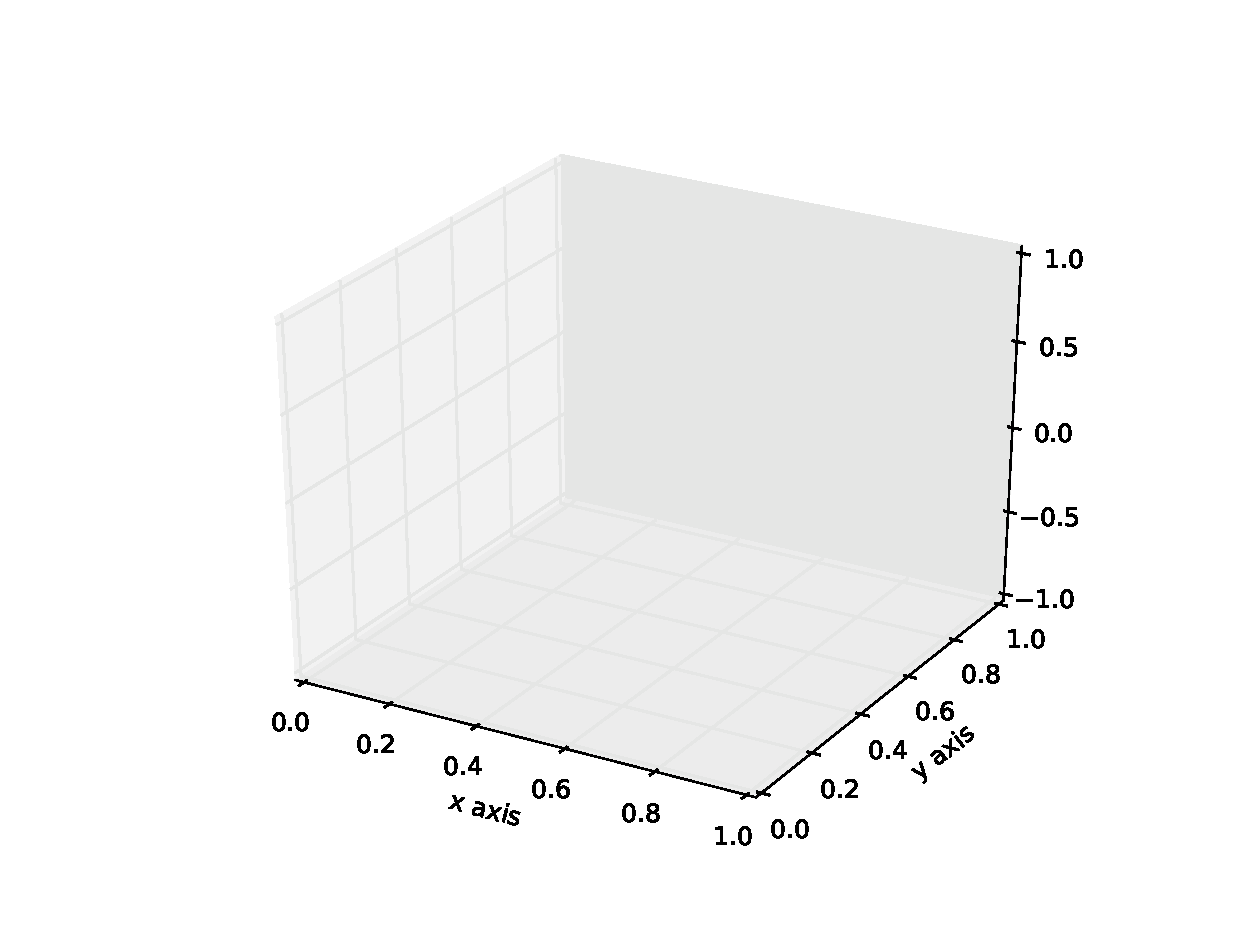
\includegraphics[scale=0.7]{Figures/InitialCondition2d.eps}
%  \caption[Initial condition in 2d]{Initial condition of manufactured solution in 2d and the simulation.}
%  \label{initial_condition_2d}
% \end{figure}

\subsection{The error estimate}\label{error_estimate}

Before we do anything we should specify what we use to measure the error which will be denoted as $\epsilon$. 
Throughout this thesis the term error is used quite lazily, but unless something else is specified we refer to the expression 
\begin{equation}
 \epsilon(t_i) = ||u_e(t_i)-u(t_i)||_2
\end{equation}
where $u_e$ is the exact (manufactured) solution to the equation, and $u$ is the result from the numerical simulation. 
We use this error-estimate because it is time-dependent, thus letting us explicitly see how the error evolves over time. 
The error is calculated over the entire mesh, letting us see clearly if the error from the random-walk areas are dominating, or (otherwise) how the PDE-scheme is holding up.
Another error estimate we will use later is the maximum value of the error. This will be used for the convergence tests to make sure that we overlook any effects of simulating for a long time. 
\begin{equation}
 \epsilon = max(\epsilon(t_i))
\end{equation}

\subsection{Verification techniques}
There are quite a few ways to verify an implementation. This thesis will focus on three which are considered adequate for no particular reason.
\begin{itemize}
 \item Method of manufactured solutions\\
 A normal way of checking that our scheme of choice is implemented correctly is by making an exact solution to the equation and checking that the error is of the expected order. 
Since the software contains both an explicit FE scheme and an implicit BE scheme they will both be verified alongside one another. 
We will start with the simplest diffusion equation (eq. \eqref{simple_diffusion_equation}) and add complexity until we have the desired expression. 
Both schemes are expected to have an error-term of the order of $\Delta t$, which in the FE case is limited by a stability criterion. 
Next, the solution to the diffusion equation is set to be equation \eqref{manifactured_solution_1D} which satisfies our equation if the diffusion constant is 1. 
\item Exact numerical solutions\\
For the explicit schemes, exact solutions to the scheme itself can be found seeing as the scheme is a difference equation. The calculations are shown step-by-step in chapter \ref{exact_numerical_solution}.
\item Convergence tests\\
This must be combined with the manufactured solution, but takes a slightly different approach to quantifying the error estimate. We start by calculating some form of error estimate, and chose a value to represent the error of the entire simulation. This could be the maximum error for the entire simulation, or an integrated measure. 
Multiple simulations will be done while improving the parameter of interest, for example how the size of the time-step influences the error. 
Finally, using equation \ref{} we get a number indicating the improvement in the error estimate by improving the parameter in question. 
This number indicates the order of convergence which is one for FE and BE since the error goes as $\mathcal{O}(\Delta t)$, and two for our approximation to the second derivative in space since the error goes as $\mathcal O(\Delta x^2)$.
A convergence rate of 1 means that halving the parameter will (roughly) halve the error, while the same reduction for a second order convergence will reduce the error by 4.
\end{itemize}


\section{Verification of PDE solvers}
To verify the implementation of the PDE-solvers we will now run through the steps outlined in the previous chapter. 
We will also add complexity along the way, but this will be described when we get there. First of all we will test the simplest possible implementation which is equation \ref{}. 
Since both the FE and BE discretization have been implemented we will test both of them, but mostly we will use the BE discretization because it has no stability criterion. 
For most of the tests we will force the solution to be equation \ref{manifactured_solution_1D} in 1d which satisfies our equation if we set the diffusion constant to 1.

Despite testing the simple cases first we will do all the tests on the same implementation (the full one) because it should be able to recreate the simple cases as well. 
Setting $D(x,y) = 0.5$ as an array with all entries equal and inserting this into the schemes will return the average of $D(x,y)$ at different mesh-points, and effectively this is the same as having only a constant. 
We will also do all verification without random walkers.

\subsection{Manufactured Solutions}

As mentioned we force the solution to be equation \ref{manifactured_solution_1D} because it fulfills the boundary conditions we have chosen.
\begin{equation}\label{manifactured_solution_1D}
 u(x,t) = e^{-t\pi^2}\cos(\pi x) +1
\end{equation}
Equations \ref{manufactured_prof_pt1} and \ref{manufactured_prof_pt2} prove that the manufactured solution we have chosen will indeed fulfill the diffusion equation (eq. \ref{simple_diffusion_equation}).
\begin{align}
 \frac{\d }{\d t}e^{-t\pi^2}\cos(\pi x) +1 &= D\frac{\d^2}{\d x^2}e^{-t\pi^2}\cos(\pi x) +1\label{manufactured_prof_pt1}\\
 -\pi^2e^{-t\pi^2}\cos(\pi x) &= -\pi^2e^{-t\pi^2}\cos(\pi x) +1 \implies 1 = 1\label{manufactured_prof_pt2}
\end{align}

The error in space is determined by two factors, the actual error caused by the approximation to the second derivative, which is of the order of $\Delta x^2$ and, in the FE case, the error term coming from the time derivative due to the stability criterion (eq. \ref{stability}), which is also of the order $\Delta x^2$. 
In 1D we get the plots in figure \ref{errorplot_FE1D_noWalk} of error described in chapter \ref{error_estimate}, with the corresponding plots of the convergence rates in figure \ref{} that verify the order of the error term.
For longer simulations, we expect the analytic solution to reach a steady state which we find in the limit of large $t$. 

\begin{equation}
 u(x,t\to\infty) \to e^{-\infty}\cos(\pi x) +1 \to 1
\end{equation}
The numerical scheme should be able to represent this to machine precision ($10^{-16}$), meaning that the numerical solution should start converging to zero after some number of times steps, but this might depend on how the derivatives as estimated so we say that it should in the very least stabilize. 
Figures \ref{} and \ref{} seem to show the expected behaviour from the error estimate, which implies that the implementation is correct so far.

\begin{figure}[H]
\centering
\begin{subfigure}[b]{0.48\textwidth}
\includegraphics[width=\textwidth]{../doc/results/experiment_31102013_1017/results/deterministic_errorplot.eps}
\caption{}
\label{errorplot_FE1D_noWalk}
\end{subfigure}
\begin{subfigure}[b]{0.48\textwidth}
 \includegraphics[width=\textwidth]{../doc/results/experiment_18112013_0830/results/deterministic_errorplot.eps}
 \caption{}
 \label{errorplot_FE1D_noWalk_long}
\end{subfigure}
\caption[Numerical error for 1D Forward Euler discretization]{Numerical error for 1D Forward Euler discretization of the PDE. Nothing else is done to the simulation.}
\label{errorplot_FE1D_noWalk_super}
\end{figure}

As we discussed in section \ref{random_walks_and_anisotropy} we should also be able to model diffusion where the diffusion constant is not a constant. 
The scheme we derived in section \ref{discretizing} already takes this into account, and so all we need to do is to add the drift term which was discussed in section \ref{effect_of_drift_on_walkers} to the scheme. 
Like before we should verify that the scheme solves the equation to the expected accuracy by using a manufactured solution \ref{manifactured_solution_1D} and tweaking the source term so this function solved the equation \ref{convection_diffusion_equation}. 
When $v=0$ and $D(x) = \pi x$ the source term becomes
\begin{align*}
 -\pi^2\exp\left(-\pi^2t\right)\cos\left(\pi x\right) &= -\pi\exp\left(-\pi^2t\right)\frac{\d}{\d x}\pi x\sin(\pi x) +f(x,t) \\
 -\pi^2\cos\left(\pi x\right) &= -\pi^2\left(\sin(\pi x) + \pi x\cos(\pi x)\right) +\tilde{f}(x) \\
 \tilde{f}(x) &= \pi^2\left(\sin(\pi x) +\cos(\pi x)(\pi x-1)\right)
\end{align*}
Once again $f(x,t) = \exp\left(-\pi^2t\right)\tilde{f}(x)$. Figure \ref{anisotropic_diffusion_verification} shows the error norm of the result of simulations of this equation with different values of $\Delta t$.

\begin{figure}[H]
\centering
\begin{subfigure}[b]{0.48\textwidth}
\includegraphics[width=\textwidth]{../doc/results/experiment_05112013_1303/results/deterministic_errorplot.eps}
\caption{}
\label{anisotropic_diffusion_verification:single_dt}
\end{subfigure}
\begin{subfigure}[b]{0.48\textwidth}
\includegraphics[width=\textwidth]{../doc/results/experiment_05112013_1304/results/deterministic_errorplot.eps}
\caption{}
\label{anisotropic_diffusion_verification:double_dt}
\end{subfigure}
\caption[Verification of anisotropic diffusion equation implementation]{Verification of anisotropic diffusion equation implementation}
\label{anisotropic_diffusion_verification}
\end{figure}
Again, the error is of the order of $\Delta t$ and is roughly halved by halving $\Delta t$.

\subsection{Convergence Tests}

The next step in testing the implementation will be to perform a convergence test in time. 
We omit the spatial convergence test because an incorrect implementation of the spatial derivative would be clearly visible both in the visualization of the simulation (the solution blows up), and in the error plot seeing as the spatial error would dominate.
We carry out the convergence test by doing several simulations with different values for $\Delta t$ and comparing the errors by equation \ref{convergence_rate_def}. 
A result of such an experiment for the FE scheme using the $\Delta t$ values listed below is found in figure \ref{convergence_test_FE}. 
The expected value of r is approximately 1. The result is not perfect, but still close to 1. 
For the BE scheme we get the convergence rate shown in figure \ref{convergence_test_BE}. Again, the expected order of convergence is 1 and this time the result is almost perfect.

\begin{equation}\label{convergence_rate_def}
 r = \frac{\ln(E_{i+1}/E_i)}{\ln(\Delta t_{i+1}/\Delta t_i)}
\end{equation}

\begin{lstlisting}
 dt = [1e-4,1e-5,1e-6,1e-7,1e-8]
\end{lstlisting}

\begin{figure}[H]
 \centering
 \begin{subfigure}[b]{0.48\textwidth}
 \includegraphics[width=\textwidth]{../doc/results/experiment_27112013_1017/results/ConvergenceTest.eps}
 \caption{Convergence test for the FE scheme. The x axis is $\ln(\Delta t)$.}
 \label{convergence_test:FE}
\end{subfigure}
\begin{subfigure}[b]{0.48\textwidth}
 \includegraphics[width=\textwidth]{../doc/results/experiment_13012014_0925_Simple1DConvergenceTestBE/results/ConvergenceTest.eps}
 \caption{Convergence test for the BE scheme. The x axis is $\Delta t$, the y-axis (though a little hard to see) is zoomed in around r=1.}
 \label{convergence_test:BE}
\end{subfigure}
\caption{Convergence tests for explicit and implicit schemes solving the simple diffusion equation (eq. \ref{simple_diffusion_equation}).}
\label{convergence_test}
\end{figure}

We can also do a convergence test, equal to the one we did in 1d, to check that the scheme converges to 1 (by equation \ref{convergence_rate_def}) for smaller $\Delta t$. 
The results of this test are shown in figure \ref{convergence_test_FE_2d} and it does converge nicely to one.

\begin{figure}[H]
\centering
\includegraphics[scale=0.7]{../doc/results/experiment_29112013_1709/results/ConvergenceTest.eps}
\caption[Convergence test FE 2d]{Convergence test for the FE scheme in 2d using $\Delta t$ ranging from the stability criterion $\frac{\Delta x\Delta y}{5}$ to the same ratio divided by 100000 in increments of $10^{-1}$.}
\label{convergence_test_FE_2d}
\end{figure}

\subsection{Exact numerical solution}\label{exact_numerical_solution}

The FE scheme also has an exact solution seeing as it is in fact a difference equation. 
We can find this (for this exact initial condition, eq. \ref{manifactured_solution_1D}) if we formulate the scheme as 

\begin{equation}
 u^{n+1} = D\Delta t u_{xx}^n + u^n
\end{equation}

and insert for the first few iterations. 

\begin{align*}
 u^1 &= D\Delta t u_{xx}^0 + u^0 \\
 u^2 &= D\Delta t u_{xx}^1 + u^1 = D\Delta t\left[D\Delta t u_{4x}^0 + u_{2x}^0\right] + u^0\\
 &= \left(D\Delta t\right)^2 u_{4x}^0 + 2D\Delta t u_{2x}^0+ u^0 \\
 u^3 &= D\Delta t u_{xx}^2 + u^2 = D\Delta t\left[\left(D\Delta t\right)^2 u_{6x}^0 + 2D\Delta t u_{4x}^0+ u_{2x}^0\right] + \left(D\Delta t\right)^2 u_{4x}^0 + 2D\Delta t u_{2x}^0+ u^0\\
 &= \left(D\Delta t\right)^3 u_{6x}^0 + 3\left(D\Delta t\right)^2 u_{4x}^0+ 3D\Delta tu_{2x}^0 + u^0 \\
 u^4 &= D\Delta t u_{xx}^3 + u^3 = \dots \\
 &= \left(D\Delta t\right)^4 u_{8x}^0 + 4\left(D\Delta t\right)^3 u_{6x}^0+ 6\left(D\Delta t\right)^2 u_{4x}^0 + 4D\Delta t u_{2x}^0 + u^0 
\end{align*}
Which we can generalize to 
\begin{equation}
 u^{n+1} = \sum\limits_{i=0}^n {n\choose i}\left(D\Delta t\right)^iu^0_{2ix}
\end{equation}
where we have
\begin{equation*}
 u^0_{2ix} = \left(-1\right)^i\pi^{2i}\cos(\pi x)
\end{equation*}
from the initial condition. This finally gives us the exact numerical solution of the FE scheme in time. 
\begin{equation}
 u^{n+1} = \sum\limits_{i=0}^n {n\choose i}\pi^{2i}\left(-1\right)^i\left(D\Delta t\right)^i\cos(\pi x)
\end{equation}

Notice that we have not used the approximation to the spatial derivative, but rather the analytical derivative. 
We find the approximation that the computer uses to the spatial derivative in the same way as for the time derivative. 
\begin{align*}
 u^0_{xx} &= \frac{1}{\Delta x^2}\left(\cos(\pi(x+\Delta x)) -2\cos(\pi x) +\cos(\pi(x-\Delta x))\right) \\
 &= \frac{2}{\Delta x^2}\left(\cos(\pi\Delta x)-1\right)\cos(\pi x)\\
 u^0_{4x} &= [u^0_xx]_{xx} = \frac{1}{\Delta x^2}\left[\frac{2}{\Delta x^2}\left(\cos(\pi\Delta x)-1\right)\left(\cos(\pi(x+\Delta x)) -2\cos(\pi x) +\cos(\pi(x-\Delta x))\right)\right]\\
 &= \frac{4}{\Delta x^2}\left(\cos(\pi\Delta x)-1\right)^2\cos(\pi x)\\
 &\dots
\end{align*}
We immediately see that this pattern continues, and we get the general formula in equation \ref{numerical_solution} for the exact numerical solution.
\begin{equation}\label{numerical_solution}
  u^{n+1} = \sum\limits_{i=0}^n {n\choose i}\left(D\Delta t\right)^i\frac{2^i}{\Delta x^{2i}}\left(\cos(\pi\Delta x)-1\right)^i\cos(\pi x)
\end{equation}
We expect the FE scheme to represent this solution more or less to machine precision, at least to $15$ digits. 
There are, however two issues with the solution \ref{numerical_solution}:
\begin{itemize}
 \item $\Delta x^{2i}$ will quickly tend to zero, and the computer will interpret it as zero. This will cause division by zero, which again ruins the simulation. This can be fixed rather simply by testing if $\Delta x^{2i}>0$ and returning zero if the test returns false.
 \item ${n\choose i}$ goes to infinity for large n and i. We will eventually (for $n>\sim170$) meet overflow. Figure \ref{convergence_exact_numerical_1d_n145} shows that at least for relatively few time steps  we can drop the troublesome terms, but effectively this limits ous simulation to some 170 steps.
\end{itemize}

\begin{figure}[H]
 \centering
 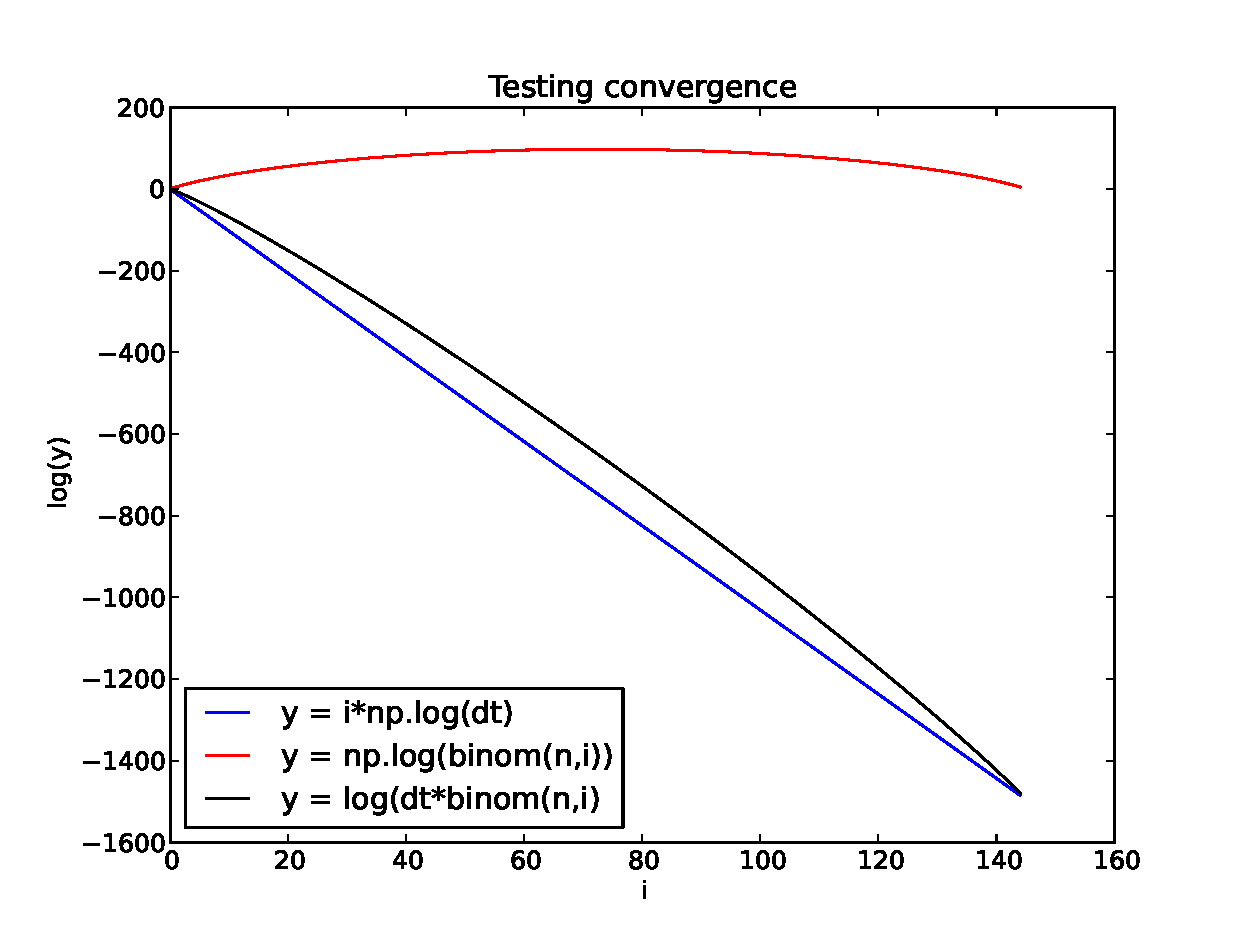
\includegraphics[scale=0.7]{Figures/convergence_exact_numerical_1d_n145}
 \caption{Testing the relation between $\left(D\Delta t\right)^i$ and the binomial coefficients.}
 \label{convergence_exact_numerical_1d_n145}
\end{figure}
The results from testing the FE scheme are found in figure \ref{errorplot_numerical_exact_FE_1D}. We see that the error in the worst case is about an order of magnitude worse than we expected. This is most likely due to the fact that we are cutting part of the solution, and over several time steps the error we do might accumulate.

\begin{figure}[H]
 \centering
 \includegraphics[scale=0.7]{Figures/exact_numerical_1d_n130.eps}
 \caption[Verification for exact numerical solution]{Error plot for 1d FE scheme compared to the exact numerical solution \ref{numerical_solution} with the modifications suggested earlier.}
 \label{errorplot_numerical_exact_FE_1D}
\end{figure}

We find the exact numerical solution to the 2d diffusion equaiton with eq \ref{initial_condition_2d_numex} as initial condition by using the same method as we did in 1d. 
The exact numerical solution of the FE scheme can be found in equation \ref{exact_numerical_solution_2d}, and again we expect the scheme to be able to reproduce this to more or less machine precision. 

\begin{equation}\label{initial_condition_2d_numex}
 u(x,y,t=0) = \cos(\pi x)\cos(\pi y)
\end{equation}

The result of a test simulation of this is shown in figure \ref{exact_numerical_2d_n130}. 
Again, as in we did in 1d, we see that although the error is very small, and start out with machine precision, it does increase and even more than in the 1d case. 
This is \emph{probably} because of the terms we have do drop in the exact numerical solution due to overflow and so on, which accumulate in the numerical solution from the scheme. 
We should, in other words, be pleased that the error starts out with machine precision, and stays small for the amount of time steps we can simulate and still have something to compare it with.

\begin{equation}\label{exact_numerical_solution_2d}
 u^{n+1} = \sum\limits^n_{i=0}{n\choose i}\left(D\Delta t\right)^i\left[2^{i-1}\cos(\pi x)\cos(\pi y)\left(\frac{(\cos(\pi\Delta x))^i}{\Delta x^{2i}} +\frac{(\cos(\pi\Delta y))^i}{\Delta y^{2i}}\right)\right]
\end{equation}

\begin{figure}[H]
 \centering
 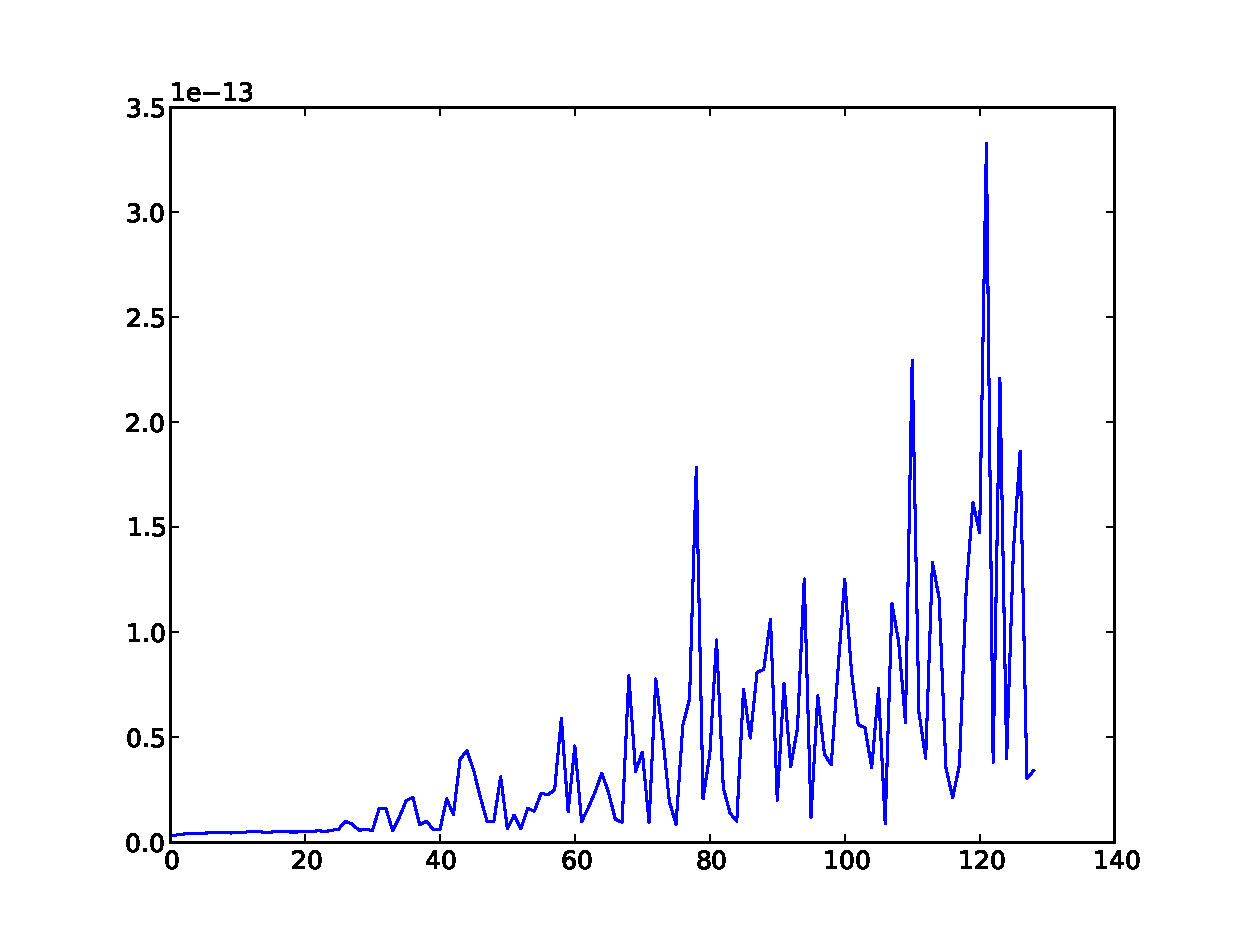
\includegraphics[scale=0.7]{Figures/exact_numerical_2d_n130.eps}
 \caption{Numerical solution from the FE scheme versus the exact numerical solution of the FE scheme in 2d. we have used a $\Delta t$ which is almost on the stability criterion, $\Delta t = \frac{\Delta x \Delta y}{5} = 8e-05$.}
 \label{exact_numerical_2d_n130}
\end{figure}

\section{Testing the Random walk implementation}\label{testing_random_walks}



To verify our implementation, and perhaps gain some new insight we will do some testing on the random walks implementation as well. 
This means that we have to find a solution of the diffusion equation \ref{simple_diffusion_equation} for an initial condition we can recreate with random walkers to the best possible precision. 
The absolute simplest initial condition to recreate is the Heaviside step function, defined in equation \ref{Heaviside_def}. 
\begin{equation}\label{Heaviside_def}
 H(x-a) = \begin{cases}
           1\;\;x\geq a\\
           0\;\;x<a
          \end{cases}
\end{equation}
In order to verify our implementation we must solve the diffusion equation \ref{simple_diffusion_equation} for this new initial condition. 
This is most easily done through separation of variables. We have
\begin{align*}
 \frac{\d u}{\d t} = D\frac{\d^2 u}{\d x^2};\;\; \frac{\d u(0,t)}{\d x} = \frac{\d u(1,t)}{\d x} = 0 \\
 u(x,0) = H\left(x-\frac{1}{2}\right);\;\; D = 1
\end{align*}
and
\begin{align*}
 u(x,t) = F(x)T(t) \implies \frac{T'(t)}{T(t)} = \frac{F''(x)}{F(x)}
\end{align*}
where the primes denotes the respective derivatives. We separate the equation using a separation constant $\lambda$
\begin{align*}
 T'(t)-\lambda T(t) = 0 \implies T(t) = C\exp(\lambda t)\\
 F''(x) -\lambda F(x) = 0 \implies F(x) = C_1\exp(\sqrt{\lambda}x) + C_2\exp(-\sqrt{\lambda}x)
\end{align*}
Where $C$, $C_1$ and $C_2$ are arbitrary constants. 
Choosing $\lambda = -\mu^2$ lets us rewrite the spatial solution in terms of sines and cosines. 
There are really three choises here; $\lambda = -\mu^2$, $\lambda = \mu^2$ and $\lambda = ?$ but we chose the former because the results of the other choises are unphysical.
\begin{equation*}
 F(x) = a\cos(\mu x) + b\sin(\mu x)
\end{equation*}
The boundary conditions gives us 
\begin{align*}
 F'(0)T(t) = F'(1)T(t) = 0
\end{align*}
Since the time dependent solution cannot be exactly zero and is independen of position by construction ($C\exp(\lambda t)|_{x=0} = C\exp(\lambda t) \neq 0$), the first derivative of the spatial solution must be zero at the boundaries
\begin{align*}
 F'(x) &= -a\mu\sin(\mu x) + b\mu\cos(\mu x) \\
 F'(0) &= -a \mu\sin(0) + b\mu\cos(\mu x) = b\mu\cos(\mu x) \implies b=0 \\
 F(1) &= a\cos(\mu) \implies \mu = n\pi
\end{align*}
Telling us that a Fourier series in cosines is the solution to the equation, and it will look like this.
\begin{equation}
 u(x,t) = a_0 + \sum\limits_{n=1}^\infty a_n\exp\left(-(n\pi)^2t\right)\cos(n\pi x)
\end{equation}

The coefficients are found by approximating the initial condition
\begin{align*}
 a_0 &= \int\limits_0^1H(x-0.5)dx = \frac{1}{2} \\
 a_n &= 2\int\limits_0^1H(x-0.5)\cos(n\pi x)dx = 2\int\limits_{0.5}^1\cos(n\pi x)dx \\
 &= \frac{2}{n\pi}\left[sin(n\pi x)\right]_{0.5}^1 = \frac{2}{n\pi}\sin(n\pi) - \sin(\frac{n\pi}{2}) \\
 a_n &= \frac{2\sin(\frac{n\pi}{2})}{n\pi}
\end{align*}
which gives us the final solution
\begin{equation}
 u(x,t) = \frac{1}{2} + \sum\limits_{n=1}^\infty \frac{2\sin(\frac{n\pi}{2})}{n\pi}\exp\left(-(n\pi)^2t\right)\cos(n\pi x)
\end{equation}
This will be the manufactures solution we will test our simulations against for the verification of the RW implemetation.

%%%%%%%%%%%%%%%%%%%%%%%%%%%%%%%%%%%%%%%%%%%%%%%%%%%%%%%%%

We can now perform a convergence test to find the convergence rate for the random walkers.
We will modify it slightly by testing for the number of walkers rather than the time step. 


Using the maximum of the error measure already in use, we have tested the convergence rate measure for the following measures of Hc:
\begin{lstlisting}
 Hc = [200,1400,5600,10400,32000]
\end{lstlisting}
The convergence test suggests that the convergence rate for random walks follows the proportionality in equation \ref{convergence_rate_RW}. 
This relation tells us just what we have been expecting the whole time; while increasing the number of walkers will reduce the error, the convergence is slow. 
Should we wish to do so, we can force the error to $\mathcal{O}(\Delta t^2)$, but this will be extremely inefficient. In fact we can find the relation as $Hc\sim\Delta t^{-2}$ for $\epsilon\sim\mathcal{O}(\Delta t)$, and $Hc\sim\Delta t^{-4}$ for $\epsilon\sim\mathcal{O}(\Delta t^2)$. Clearly we will have enough trouble for the simpler cases.

\begin{equation}\label{convergence_rate_RW}
err \propto Hc^{\frac{-1}{2}}
\end{equation}


\begin{figure}[H]
 \centering
 \includegraphics[scale=0.7]{../doc/results/experiment_18022014_1413_RW_convergencetest_1d/ConvergenceTest.eps}
 \caption[Convergence test RW]{A convergence test for the isotropic random walk implementation using different conversion factors, Hc. The x axis (conversion rate) is log transformed and ranges from 100 to 50000 in real numbers.}
 \label{ConvergenceTestRW}
\end{figure}
\begin{figure}[H]
 \centering
 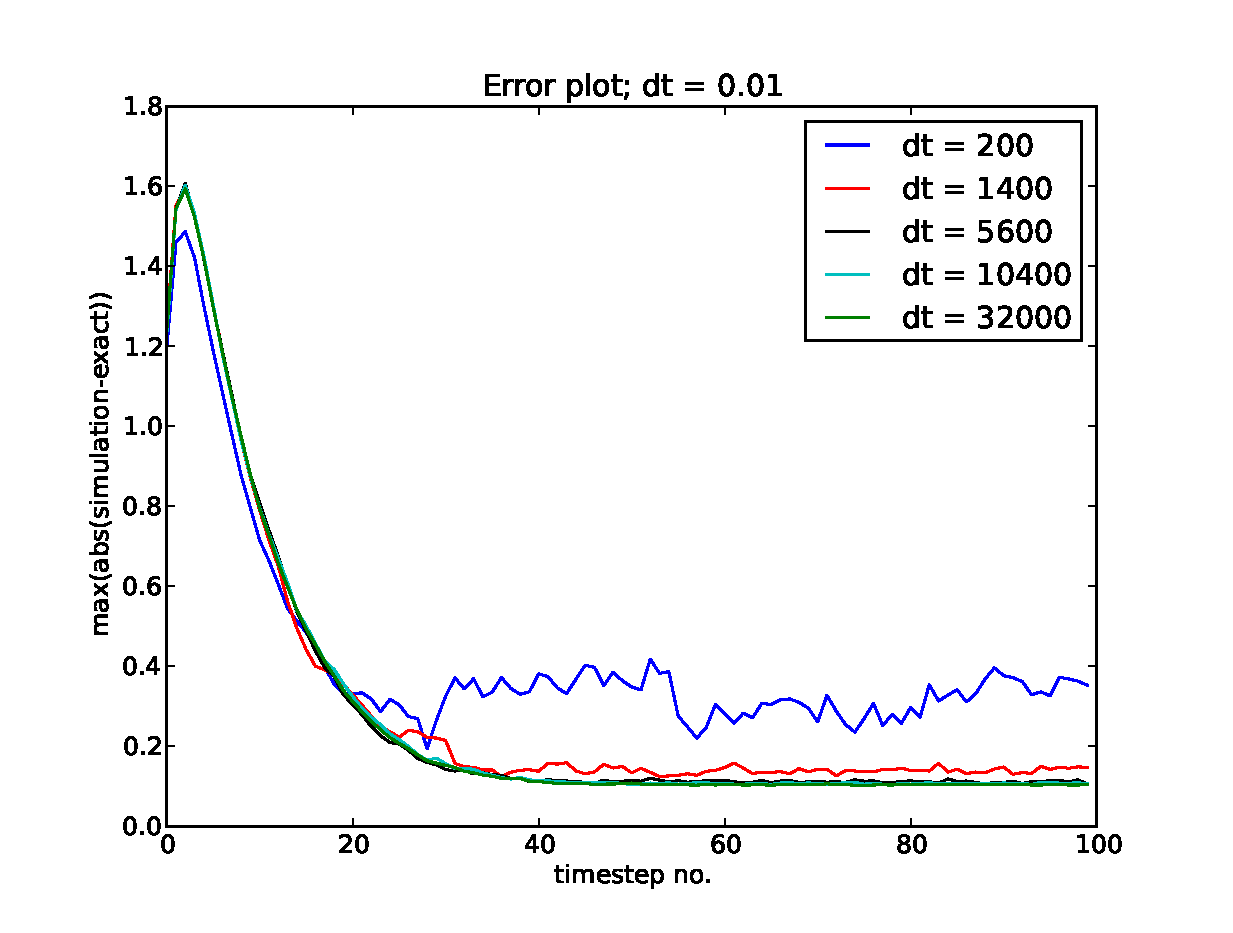
\includegraphics[scale=0.7]{../doc/results/experiment_18022014_1413_RW_convergencetest_1d/results/errorplot.eps}
 \caption[Error plot RW]{A ``normal'' error plot for the same simulation as in figure \ref{ConvergenceTestRW}. The $\Delta t$ in question is used to couple the RW simulation and the exact solution. For each $\Delta t$ the RW simulation does 100 steps with a step length calculated from equation \ref{steplength}}
\end{figure}




\section{Testing the combined solution}
In this chapter we will combine the PDE-solution on some part of the mesh with the result from a random walk simulation using the same initial condition as the PDE-solver was given. 
As we will discuss in chapter \ref{Software:About} there are many candidates as to the combination of the solutions, but we will use one of the simplest ones; the average of the two. 
Before we start with the verification, however, we will take a quick look at a simplified problem which in principle is the same.

\subsection{A simplified version of the algorithm}\label{simplified_test}

Monte Carlo methods are immensely important in modern computational science (\emph{reference}), and can be used to solve integrals as well as random walks. 
As a simplified analogy to our method for solving the diffusion equation we ca look to the Ordinary Differential Equation (ODE) in equation \ref{ODE}. 
\begin{equation}\label{ODE}
 \frac{\d f}{\d x} = a(x)\;\text{,}\; x\in [a,c]
\end{equation}
Equation \ref{ODE} is easily solvable (see eq. \ref{ODE_solution}). For the sake of illustration we also specify that $a(x) = \frac{1}{x}$ and divide the integral in two parts, introducing $b\in (a,c)$.
\begin{equation}\label{ODE_solution}
 f(x) = \int\limits_a^b a(x)\,dx + \int\limits_b^c a(x)\,dx
\end{equation}
This is a case where we have complete control over all parts of the solution which is $f(x) = f(b)-f(a) + f(c)-f(b)$, and we can solve the two parts of the integral in two different ways; by the midpoint method and by MC integration. The convergence rates of these methods are $2$ and $0.5$ respectively. 
By the relation we found in chapter \ref{} (eq. \eqref{definition_Hc_first}) the number of MC samples should be proportionate to the resolution used by the midpoint-rule to the power of four. 
\begin{align*}
 \frac{1}{\sqrt{N}} \simeq \Delta x^2 \\
 N \simeq \frac{1}{\Delta x^4} = N_x^4
\end{align*}
The following output is from a program generously donated by Hans Petter Langtangen which does the required integration and calculates the convergence rates. 
It uses the relation described, but multiplies with a constant, giving us 
\begin{equation}\label{num_walkers_MC_integration}
 N = 2000\times N_x^4
\end{equation}

\begin{lstlisting}
  N_x	    N_MC	   error       MC_error   MP_error
   1        2000 (   1)  2.650E-02   2.648E-02   2.391E-05
   2       32000 (   1)  7.392E-03   7.433E-03  -4.136E-05
   4      512000 (   1)  1.918E-03   1.927E-03  -8.954E-06
   8     8192000 (   8)  4.683E-04   4.866E-04  -1.832E-05
  16   131072000 ( 131)  1.176E-04   1.220E-04  -4.320E-06
  
  Convergence rates
total  MP     MC
-1.84 -1.83  0.20
-1.95 -1.95 -0.55
-2.03 -1.99  0.26
-1.99 -2.00 -0.52
\end{lstlisting}
We see that the convergence rate for the whole integral is roughly $2$ which is what we expect. This suggests that the idea behind the algorithm is sound. \\
Another thing to notice it the convergence rate of the MC method which is sort off all over the place, this illustrates how difficult it is to verify the simulations. 
As the listed output and equation \ref{num_walkers_MC_integration} shows, the number of walkers or MC samples grows very fast making it computationally very demanding to do the calculations.

\subsection{Introducing walkers}

First of all, using random walkers on parts of the mesh will have a considerable, negative impact on the error estimate. 
As we have discussed before, the solution from the random walkers will fluctuate around the ``correct'' (it is in fact correct while verifying) solution with amplitude proportional to $\frac{1}{\sqrt{N_{ij}}}$ which will depend on the PDE-solution in the mesh-point. 
It will also, as demonstrated in chapter \ref{simplified_test}, be possible to force the combined solution to have the desired properties in terms of error-estimates but at considerable computational cost. 
While doing the various error-testing for the combined solution we will therefore stick to the implicit scheme since we can choose the time-step more freely and by extension reduce the number of random walkers required.\\
Keeping in mind that the spatial error goes like $\Delta x^2$ we should at least choose the time-step so that $\Delta t> \Delta x^2$ to make sure the error from the time derivative is dominant. 
Starting off, we have a 2d simulation of isotropic diffusion with $\Delta t = 0.01$ and $\Delta x = \frac{1}{75}$ over the full interesting course of the solution, meaning that the solution more or less at steady state the last time-steps. The error-plot from this simulation is shown in figure \ref{errorplot_combined_BE2d}. We can see that although the error-term from the combined solution does not converge onto the error-curve from the deterministic solution, the error term is of the same order. 
\begin{figure}[H]
 \centering
 \includegraphics[scale=0.7]{../doc/results/experiment_17022014_1541/results/errorplot.eps}
 \caption{Error-plot of the combined solution using an increasing number of walkers. Parameters of importance are $\Delta t = 0.01$, $\Delta x = \frac{1}{75}$. Simulations doen with the BE scheme for 100 steps.}
 \label{errorplot_combined_BE2d}
\end{figure}

%%%%%%%%%%% Cut this %%%%%%%%%%%%%%%%%%%%%%%%%

We then introduce an area on the domain where we switch models from the normal PDE to an average of the PDE solution and the result of a random walk simulation where the initial condition is the last time step from the PDE converted to walkers by the conversion rate given in equation \ref{conversion_rate}. In this case we have used the parameters $a=3$, $\Delta t = \frac{\Delta x^2}{3.0}$, $\Delta x = \frac{1}{20}$. 
These parameters makes one unit of $u(x,t)$ equal to some $1000$ walkers. 
\begin{equation}\label{conversion_rate}
 C_{ij} = \frac{a}{\Delta t}U_{ij}
\end{equation}
Mostly we will rewrite equation \ref{conversion_rate} to just one conversion factor times the PDE solution, giving us some flexibility should we want to add more dependencies in the conversion. 
As of now, the conversion factor, $Hc$, is defined in equation \ref{definition_Hc_first}. 
One ``unit'' of $ U_{ij}$ will directly correspond to $Hc$ random walkers.
\begin{equation}\label{definition_Hc_first}
 Hc =  \frac{a}{\Delta t} \implies C_{ij} = Hc\cdot U_{ij}
\end{equation}
%%%%%%%%%%% And paste somewhere smart %%%%%%%%%%

\subsection{Increasing the time step and the relative size of walk-area}\label{increasing_dt}

Now that we have an estimate of how to adjust the step length of the walkers in order to adjust for the time step, $\Delta t$, on the PDE level we would like to investigate the actual effects of running the simulation with a larger time step to verify our calculations. 
First off all, figure \ref{errorplot_BE1D_noWalk} shows the error norm of a simulation of the simplest diffusion equation \ref{simple_diffusion_equation} discretized by the Backward Euler scheme \ref{BE_discretisation_isotropic} using a time step which would make the Forward Euler discretization unstable (There is something strange about its convergence). 
Figure \ref{errorplot_BE1D_Walk} shows the same simulation for various conversion parameters for the random walk. 
These simulations have input from the random walk model on some 20\% of the mesh points. 
As a comparison we can turn to figures \ref{errorplot_BE1D_walk_5_percent} and \ref{errorplot_BE1D_walk_35_percent} which have 5\% and 35\% of the mesh points affected by walkers.

\begin{figure}[H]
\centering
\begin{subfigure}[b]{0.48\textwidth}
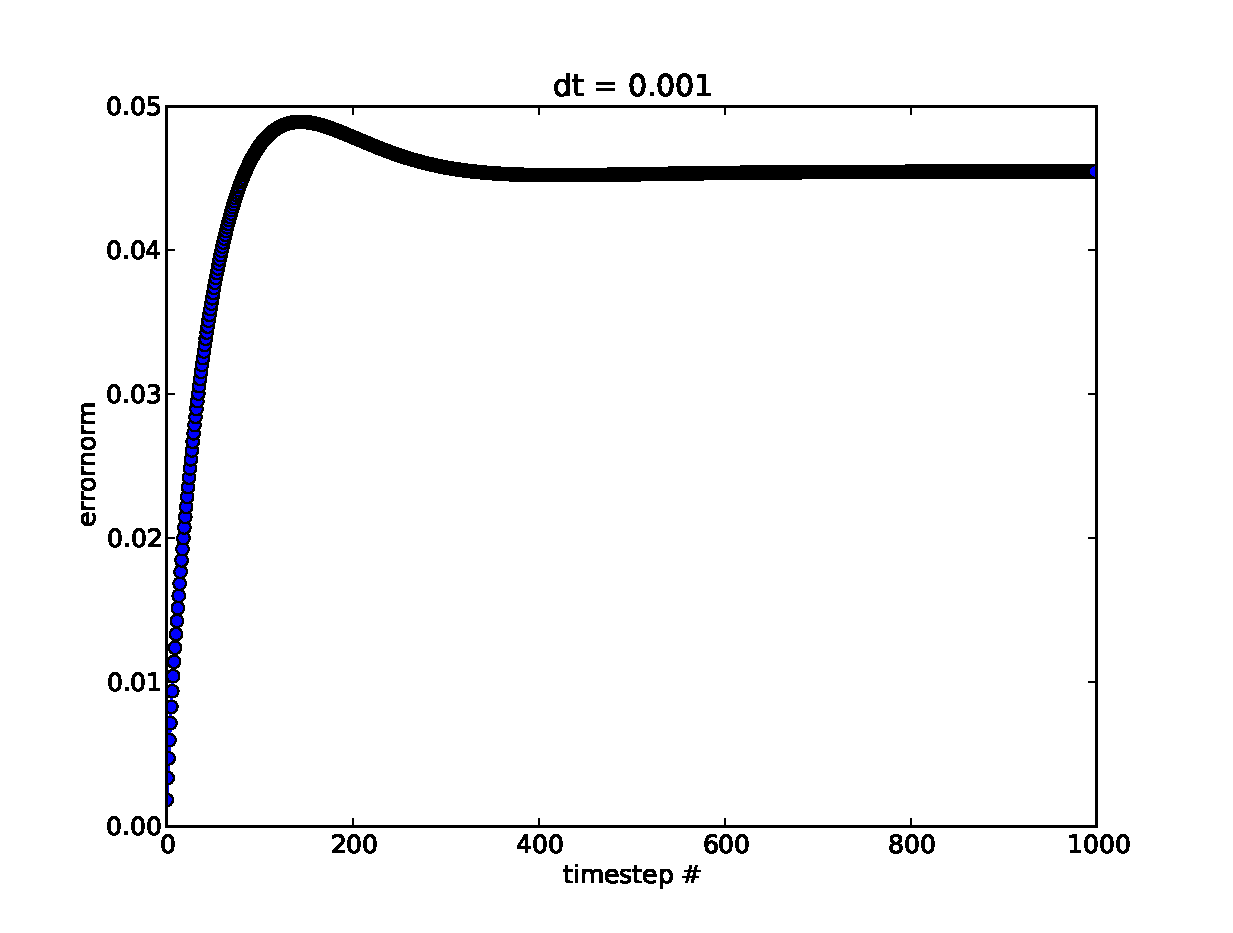
\includegraphics[width=\textwidth]{../doc/results/experiment_19112013_1514/results/deterministic_errorplot.eps}
\caption{}
\label{errorplot_BE1D_noWalk}
\end{subfigure}
\begin{subfigure}[b]{0.48\textwidth}
 \includegraphics[width=\textwidth]{../doc/results/experiment_19112013_1514/results/errorplot.eps}
 \caption{}
 \label{errorplot_BE1D_Walk}
\end{subfigure}
\caption[Numerical error for 1D Backward Euler discretization]{Numerical error for 1D Backward Euler discretization of the PDE. In figure b there has been added walkers to the solution in the area $x\in[0.5,0.7]$.}
\label{errorplot_BE1D_first}
\end{figure}

\begin{figure}[H]
\centering
\begin{subfigure}[b]{0.48\textwidth}
 \includegraphics[width=\textwidth]{../doc/results/experiment_19112013_1559/results/errorplot.eps}
 \caption{Having walkers on 5\% of the mesh points.}
 \label{errorplot_BE1D_walk_5_percent}
\end{subfigure}
\begin{subfigure}[b]{0.48\textwidth}
 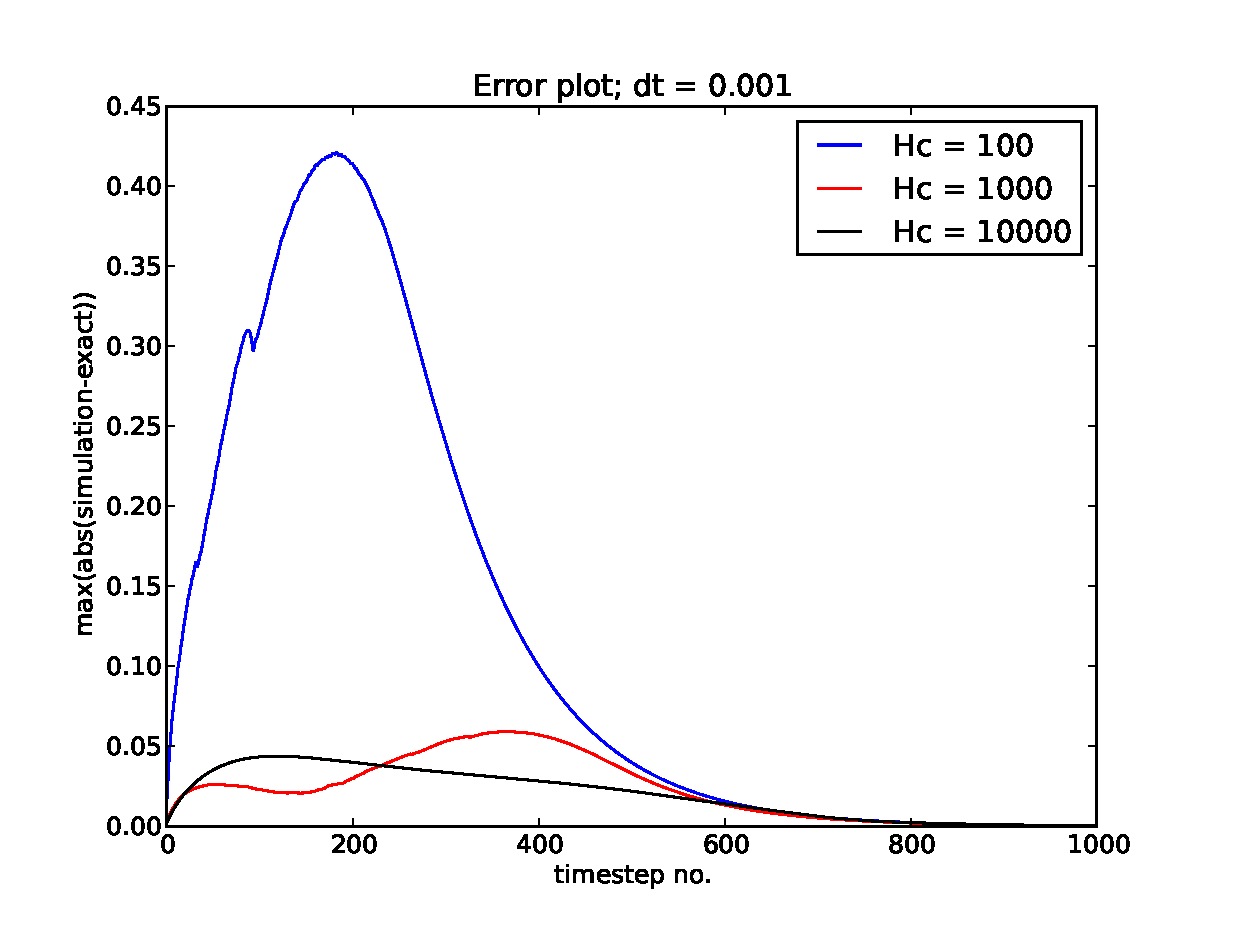
\includegraphics[width=\textwidth]{../doc/results/experiment_19112013_1603/results/errorplot.eps}
 \caption{Having walkers on 35\% of the mesh points.}
 \label{errorplot_BE1D_walk_35_percent}
\end{subfigure}
\caption{The effect of increasing the size of the walk area for a fixed $\Delta t = 0.001$ using the BE discretization.}
\label{testing_walk_area_size_BE}
\end{figure}

These experiments have been done using the Backward Euler discretization so that we can simulate for a longer time and still see the effects to their full extent. 
We have also investigated the effects of changing the time step (also using the BE discretization to avoid instabilities and be able to do longer simulations). 
The results are summarized in figure \ref{testing_dt_size}. 
We notice something a bit unexpected in figure \ref{errorplot_BE1D_walk_large_dt}. 
Unlike almost all the other comparable plots, it seems that using the least amount of walkers gives the best result here. 
This might be because the system quickly reaches its steady state, and will then be very well described by the continuum model. 
Having a small conversion factor, Hc, will mean that very quickly there will be no walkers which sort of ruins the point. 
This particular equation has steady state $u(t\to\infty,x) = 0$, and so not having any walkers will be perfect. What we should read from this figure is rather that the simulation with the most walkers converges to an acceptable error, and that this is achieved just as fast as for the other two simulations.



\begin{figure}[H]
\centering
\begin{subfigure}[b]{0.48\textwidth}
 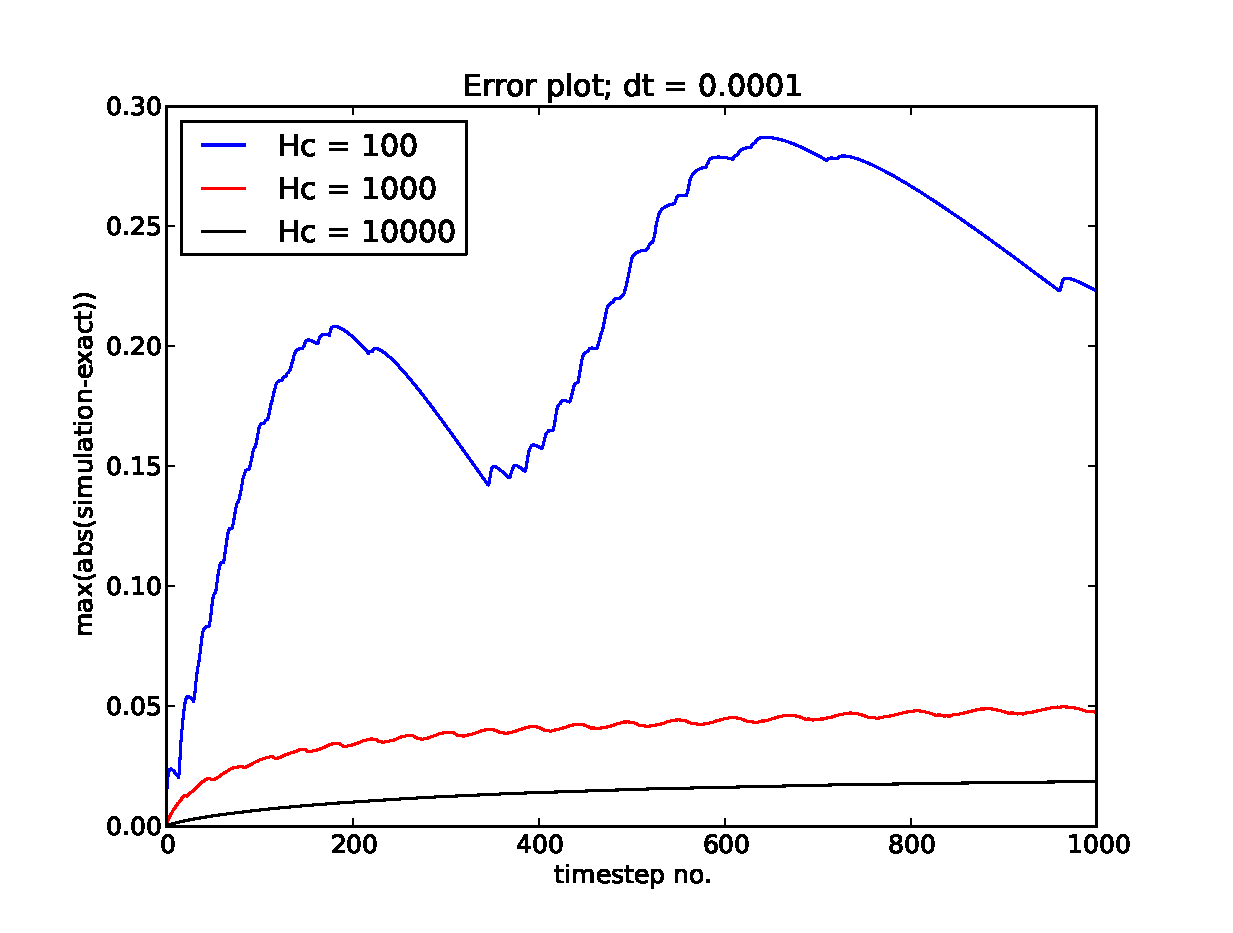
\includegraphics[width=\textwidth]{../doc/results/experiment_19112013_1625/results/errorplot.eps}
 \caption{Using a normal $\Delta t = 0.0001$.}
 \label{errorplot_BE1D_small_dt}
\end{subfigure}
\begin{subfigure}[b]{0.48\textwidth}
 \includegraphics[width=\textwidth]{../doc/results/experiment_19112013_1627/results/errorplot.eps}
 \caption{Using a large $\Delta t = 0.01$.}
 \label{errorplot_BE1D_walk_large_dt}
\end{subfigure}
\caption{}
\label{testing_dt_size}
\end{figure}

\begin{figure}[H]
 \centering
\begin{subfigure}[b]{0.48\textwidth}
\includegraphics[width=\textwidth]{{../doc/results/experiment_02122013_1309_long_simulations_1d/results/errorplot}.eps}
 \caption{}
 \label{errorplot_FE_walk_long:normal}
\end{subfigure}
\begin{subfigure}[b]{0.48\textwidth}
 \includegraphics[width=\textwidth]{{../doc/results/experiment_02122013_1309_long_simulations_1d/results/deterministic_errorplot}.eps}
\caption{}
\label{errorplot_FE_walk_long:deterministic}
 \end{subfigure}
\caption[Errorplot, long simulation]{The deterministic error and the error from simulations with walkers for long simulations.}
\label{errorplot_FE_walk_long}
\end{figure}



\chapter{Software}
\section{About}

\section{Adaptivity}
There are two adaptive parts of the software. First of all, the number of walkers which depend on the concentration, or the solution the the PDE in the relevant area. This must change in order to keep physical meaning and give results. Without this adaptivity, the results would either be wrong, or the model would not make physical sense.\\
Since a diffusion process in general has rapid changes in the beginning where for example high frequency variations are dampened and very slow convergence to a steady state later, we have introduced a test of the amount of change between two subsequent time-steps. If this amount is smaller than some limit, we will increase the time-step.\\
\emph{This increase should be done in a more elegant manner(linearly?)}

\section{Computational cost}
This chapter will consider the expensive parts of the code and look at possible improvements.

\subsection{Memory}
The memory-expensive parts of the code include storing the decomposed matrices, and storing the random walkers.

\subsection{CPU time}
There are four expensive operations in the algorithm as it stands now with the BE discretization using standard LU-decomposition.
\begin{itemize}
\item Performing the LU decomposition is very expensive. There might be a way to make this step more efficient by utilizing the sparsity of the linear system.
\item The cost of solving the PDE increases drastically with the spatial dimension, at least as long as we use an implicit scheme. The FE scheme will actually save us $d$ orders of operations in $d$ dimensions, at least with the BE discretization using the standard LU decomposition. If we could utilize some specialized Gaussian elimination like the one we have for tridiagonal matrices we might be able to improve this.
\item Random walks are expensive if there are many walkers. The number of calls to the random number generator follows eq. \ref{calls_to_ran} and for the verification process, which required a lot of walkers, this represented a considerable cost.
\item De- and re-allocation of random walkers each time-step is also an immensely costly procedure. An alternative might be to keep the number of walkers constant and rather change the conversion-factor, Hc, although this approach sacrifices physical meaning.
\item Writing the results to file will require $\mathcal{O}(n^d)$ operations where the operations are quite slow. We can get some speed-up by writing in binary, but as of now it has proved problematic to make python interpret the result-files. 
\end{itemize}

\begin{equation}\label{calls_to_ran}
 N_{\text{calls}} \propto Hc\frac{(x_1-x_0)}{\Delta x}\frac{(y_1-y_0)}{\Delta y}\tilde{T}
\end{equation}
where $\tilde{T}$ denotes the number of timesteps on the PDE level times the number of time-steps one PDE-step corresponds to on the RW level. Note that this expression will NOT be zero in 1d, and that it is dependent on the PDE-solution.

\subsection{Parallelizability}
In the final algorithm there are the following stages
\begin{itemize}
 \item Initialization\\
 Read parameters from command-line, initial condition and diffusion ``tensor'' from file. Setup instances of solvers etc. Practically no point in parallelizing this.
 \item LU-decomposition\\
 The actual LU-decomposition is a sort of Gaussian Elimination which is costly ($\mathcal{O}(N^3)$). Although the decomposition is pre-implemented at this point, the plan is to implement my own version of this. This step should be possible to parallelize.
 \item Solving\\
 This step includes a back-transform of the decomposed matrix which is expensive for $d>1$. This step should be parallelizable. It also includes the random walk part which is both expensive (depending on the number of walkers left) and highly parallelizable. We also write stuff to file which is quite costly. This is probably not possible to parallelize.
\end{itemize}

Parallelization of the random walk solver should scale linearly because the only form of communication required is shared memory. 
The LU decomposition and back-substitution require some communication and will not scale linearly, but will still benefit from parallelizing. 



\chapter{Results}
\section{Results of verification}
This section will quickly summarize the results of chapter \ref{chapter:analysis} and \ref{chapter:application}.


\subsection{The FE scheme}
Although not all of the results from verification of the FE scheme are perfect, the results from testing the exact numerical solution are really good. 
The numerical exact solution test is a verification of the implementation of the FE scheme. 
A successful test indicates that the scheme is correct and will solve the diffusion equation to the expected accuracy. 
When the convergence tests for the FE scheme could be better it is most likely due to other effects like not being able to make the error from the spatial derivative sufficiently dominant. 
The result of verifying the FE scheme is that it is deemed correctly implemented within the limits of the applied tests.

\subsection{The BE scheme and the block tridiagonal solver}
Most of the tests done on the BE scheme are close to perfect. 
Only when testing the scheme versus the numerical exact solution are the results slightly off. 
Though the numerical exact solution test is expected to give an error close to machine precision the results are five orders of magnitude larger than machine precision. 
On the other hand, the error term is also eight orders of magnitude smaller than the time step and there are a lot of possible round off errors in the inverted coefficient matrix which can explain the lack of accuracy. \\
Effectively, testing the convergence rate also verifies the assembly of the coefficient matrix while testing against the numerical exact solution verifies that the block tridiagonal solver works properly.\\
The result of verifying the BE scheme is that both the assembly of the coefficient matrix (and by extension the discretization of the diffusion equation) and the block tridiagonal solver are deemed correctly implemented. 

\subsection{The RW solver}
Due to fluctuations in the solution it is hard to get a good convergence rate for the RW solver. 
However it is measured to be close to $0.5$ both with respect to the time step and wit respect to the number of walkers introduced. 
% Seeing as there is no exact numerical solution for a random walk, only statistical properties 
The result of verifying the RW solver is that it is deemed correctly implemented within the limits of the applied tests.

\subsection{The hybrid diffusion solver}
For this thesis it is considered very important that the hybrid diffusion solver can have first order convergence in time if the conversion rate is high enough. 
As Figure \ref{combined_BE1d:convergence} shows this was achieved, and the hybrid solver is therefore considered adequately implemented for the time being.\\

Effects of varying the relative size of the RW area were also illustrated. 
The result of increasing the portion of the PDE mesh affected by an RW model is clearly a larger error term overall, while decreasing the size of the RW area significantly improves the error term. 
All of this is expected since more fluctuations are introduced.

\section{Results for physical application}

Craske et.al. suggest that the neck of spines act as diffusion barriers which slow down, but don't completely stop the diffusion of PKC$\gamma$ into spines. 
The function of this barrier is a bit unclear, but the presence of it is undisputed. 
In their measurements they found a delay of around $5-10$ seconds from elevated concentration levels in the dendrite until a similarly elevated concentration level occurred in spines with necks longer than $0.5\mu$m. 
Using parameter values which resemble the values found in actual (rodent) neurons and neurites in the developed software, the observed delay-times have been recreated. 
Figure \ref{results:spine_diffusion_stats} shows plots of the observed diffusion times into spines. 
This figure shows a clear trend for longer diffusion times as the neck length of the spine increases. 
Figure \ref{results:boxplot_relative_diffusiontime_long_neck} further support this claim and implies the average diffusion time for PKC$\gamma$ into long necked spines to be of accordance to the results from Craske et.al.
Seeing as there are no additional complexities added to the random walk model we can assume that the spine neck does in fact function as a diffusion barrier.

\begin{figure}[H]
 \centering
\begin{subfigure}[b]{0.48\textwidth}
 \includegraphics[width=\textwidth]{Figures/spine_stats_fulltime_nl.eps}
 \caption{Absolute diffusion times.}
 \label{results:spine_diffusion_stats:fulltime}
 \end{subfigure}
 \begin{subfigure}[b]{0.48\textwidth}
 \includegraphics[width=\textwidth]{Figures/spine_stats_reltime_nl.eps}
 \caption{Relative diffusion times.}
 \label{results:spine_diffusion_stats:reltime}
\end{subfigure}
\caption[Diffusion times with least squares fit]{Absolute (a) and relative (b) diffusion times into spines. The lines represent a least squares fit of the results. This least squares fit should have been done after removing outliers and should have an expression written out somewhere.}
\label{results:spine_diffusion_stats}
\end{figure}

\begin{figure}[H]
 \centering
 \includegraphics[scale=0.5]{Figures/spine_stats_boxplot_reltime_longneck.eps}
 \caption[Diffusion time for long necked spines]{Boxplot of the relative diffusion times (time between elevated concentration in dendrite and elevated concentration in spine head) into spines with necks longer than $0.5\mu$m. Similar studies were done by Crase et.al. and found diffusion time (unclear whether relative or not) to be somewhere around 5-10 seconds.}
 \label{results:boxplot_relative_diffusiontime_long_neck}
\end{figure}

Through the simulations it became apparent that there must be some sort of limiting factor which limits the number of PKC$\gamma$ particles that are let into the spine. 
In real life this is achieved by a concentration gradient which tends to zero (or negative values) meaning that no particles will diffuse into the spine after it is ``filled'' up. 
A random walker will not feel this concentration gradient unless it is explicitly told so. 
The alternative solution then, is to reduce the probability for particles to diffuse into a spine for each particle that get caught in the spine head by a factor $\frac{1}{10}$. 

\appendix
\chapter{}
\section{Debugging}\label{debugging}

In any project which involves programming one is bound to do some debugging. This project is no exception. 
Debugging can be extremely frustrating because no one sees all the hours that go into finding the bugs. 
Should a bug not be found, however, it will be noticed immediately. 
This appendix is an introductory guide to debugging finite difference (FD) solvers and RW implementations. It starts out with some general tips on how to handle error messages, and moves on to deal with FD and RW implementations. 
Finally, some words on how to debug the developed software are included.

\subsection{Compiler/syntax errors}
If you are programming in a compiled language like Fortran or C/C++ it is very easy to forget or misspell some syntax. 
Usually, the compiler will tell you what is wrong. 
Should it not do so, there are compiler options which provide extra information about syntactically correct but questionable looking code (-Wall). 
Some times one error results in several error messages. 
Start with the messages that are understandable, and recompile before checking out the other messages. \\

\noindent If you are building a larger project which requires linking, remember that packages must be linked in the correct order. 
For example; the Armadillo linear algebra library is backened by LAPACK and BLAS. 
In addition to linking the Armadillo library, both LAPACK and BLAS must be linked, and they must be linked in the correct order: 
\begin{lstlisting}
 g++ myprog.cpp -o myprog -O2 -larmadillo -llapack -lblas
\end{lstlisting}
Anything else will give very cryptic compiler errors. \\

Interpreted languages, like Python or MatLab, mostly include debuggers which provide extensive information about any errors in the code, read them thoroughly.

\subsection{Segmentation faults}
Segmentation fault is a very common abort message to get from C++. It means that the program has tried to access a part of the computer memory (RAM) which it is not allowed to access by the operating system. 
Interpreted languages will abort with a more informative error message, saying something about where the error was encountered. 
In a compiled language, ``Segmentation fault'' is all you get, which basically means that there is something wrong somewhere in your code. 
As an illustration, the terminal output below shows the output from a python- and C++- program (both named ``segfault'') for the same error:
\begin{lstlisting}
fredrik@Workstation:~/uio$ python segfault.py 
Traceback (most recent call last):
  File "segfault.py", line 3, in <module>
    b = sys.argv[1]
IndexError: list index out of range

fredrik@Workstation:~/uio$ ./segfault 
Segmentation fault (core dumped)
\end{lstlisting}

The gnu-compiler has an environment called gdb in which you can run your program. 
``gdb'' will catch segmentation faults and provide some information about where they were encountered. 
Furthermore, advanced editors like ``qt creator'' have built-in debuggers and the ability to place breakpoints in the code, making it possible to step through code line by line. \\
Some times though, the thing that works best is to print messages or key values at various places, signaling that a code block is finished. 
For example, making each function print its name when it is called will quickly identify problems. 

\subsection{Finite difference methods}
First and foremost: Do the discretization by hand. 
It will give valuable insight, which makes implementation and debugging a lot simpler. 
Secondly, the numerical stability of the scheme should be investigated prior to implementation. 
This ensures that a conditionally stable scheme does not fail tests because of a to large discretization parameter. \\

\noindent There is one very important rule in programming in general: ``First make it work, then make right, then make it fast''. 
When solving PDEs numerically this principle is extra important. 
A numerical discretization scheme will (to my knowledge) either result in a main loop or a linear system which solves the equation. 
Regardless of the overall structure of the final program, this main block will be located unchanged somewhere within the final structure. 
This part should therefore be implemented and tested first. 
Structural changes and efficiency issues can be addressed at a later point. \\


\noindent Visualization is an invaluable tool while implementing a numerical PDE solver. 
Even though the code runs through all the steps without crashing, it does not have to be correct. 
This is illustrated in Figure \ref{appendix:visual_debugging}.
\begin{figure}[H]
 \centering
 \begin{subfigure}[t]{0.48\textwidth}
  \includegraphics[width=\textwidth]{Figures/incorrect_implementation.eps}
  \caption{Incorrect implementation}
 \end{subfigure}
 \begin{subfigure}[t]{0.48\textwidth}
  \includegraphics[width=\textwidth]{Figures/correct_implementation.eps}
  \caption{Correct implementation}
 \end{subfigure}
 \caption[Visual debugging]{Illustration of an implementation which does not crash the program, but is still clearly incorrect (a). (b) shows the correctly implemented version of the same time step.}
 \label{appendix:visual_debugging}
\end{figure}

 
\noindent At this point I would like to introduce rubber-duck debugging which is said to be invented by Dennis Ritchie, the developer of the C programming language. 
The story goes that he would keep a rubber duck at his desk and whenever he was stuck, would describe the code in detail (what each statement did and was supposed to do) to the rubber duck. 
Asking questions, and saying thing out loud forces you to think about things in a slightly different manner. \\

\noindent When the code seems to reproduce the intended results it is time to start the verification. 
This is where we make an error estimate and do some numerical analysis. 
Making sure an implementation is correct is a lot harder than it sounds, but there are a few points that should be fulfilled:

\begin{itemize}
 \item Manufactured solution\\
 As was described earlier, the source term of the equation can be used to force almost any solution upon the equation. 
 
 \item Stationary solution\\
 This is a special type of manufactured solution. Using the source term, and initial condition, the solution can be forced to be constant. 
 If a scheme reproduces a stationary solution it conserves energy, which is very desirable.
 \item Exact numerical solution\\
 Depending on the discretization, it should be possible to find an exact solution to the discretized version of the PDE. 
 An example of this is found in chapter \ref{exact_numerical_solution}. 
 The scheme is expected to reproduce this solution to machine precision, but there are often several factors which limit the accuracy. 
 At the very least, the error should be significantly smaller than the largest error term. \\
 \item Convergence test\\
 It is often difficult to make convergence tests work properly, but they are arguably the most powerful tests and therefore important to implement. 
 The principle is to verify that using a smaller discretization parameter results in a smaller error, and that the error is reduced by the expected amount. 
\end{itemize}

\noindent There are probably more ways to make sure that a finite difference scheme is working properly, but the ones listed will usually give a good implication.

\subsection{Random Walk and Monte Carlo methods}

While solving a PDE numerically, the intermediate calculations can be checked and verified. 
Since Monte Carlo methods are based on random numbers, the results of intermediate calculations will be random, making it impossible to verify them completely. 
Instead, some statistical properties of the random numbers can be verified. 
For example, using uniformly distributed random numbers will give a certain mean and standard deviation, while a Gaussian distribution will give another.
The random number generator should be tested in order to verify that these properties are reproduced to a reasonable accuracy. \\

\noindent Random walkers have some additional properties which can be tested. 
Both a one-dimensional and a two-dimensional random walk will fill all available space, given infinitely many time steps. 
Letting 4-5 walkers jump around for around $10^4$ time steps, and plotting their paths should give an indication of how well this property is reproduced. \\

\noindent Finally, it is very useful to specify a random seed. This will ensure that the random number generator produces the same sequence of numbers each simulation, which often makes testing easier. 
 
% As we have discussed earlier the fluctuations in a MC-model are usually of a magnitude $\frac{1}{\sqrt N}$ this is also smart to verify. \\
% Finally, you should absolutely have the possibility to set the random seed and check that two runs with the same random seed produces the exact same result and makes sure you are using a RNG with a large enough period. The xor-shift algorithm by Geroge Marsagla \cite{} has a period of around $10^{48}$ which usually is more than adequate.

\subsection{The developed software}

Since the developed software combines two solvers, it is of course very important to make sure that each solver is working properly. 
This can be verified by performing the tests mentioned earlier. 

While implementing the hybrid solver, there were four main points which either made the work easier, or would have made the work easier:

\begin{itemize}
 \item Unit testing\\
 This is a way to test a single unit of code, often a single function, and verify that it does exactly what it should do. \\
 \item Version control\\
 During implementation and testing, a lot of changes will be made to the code. It is surprisingly difficult to remember all the changes, which often means that functioning code will be lost. 
 Using version control software eliminates this problem. Version control software allows a developer to save snapshots of code with a comment, as well as some more advanced options. This allows for tracking of progress, committing working code before changes are made, and much more. Should some changes be made to a working piece of code, it can be reverted to the last working version.\\
 \item Make independent modules\\
 This applies to most code development. If the code is divided into independent modules, it is not only easier to test the code, it will also be much easier to reuse the code. \\
 As an example, the block tridiagonal solver has been implemented as a separate module, which since then has been used by Torbjørn Sæland in his masters thesis.\\
 \item Do not be nostalgic\\
 Because you are now using version control, there is no need to comment out sections of code in case it is needed later. 
 This makes the rest of the code less messy, and reduces the risk of forgetting to remove something.
\end{itemize}

% 
% For some 2 months while working with this project I got really good results which seemed to verify all the important parts of the theory. 
% Unfortunately it turned out that, while individually both parts of the program did exactly what they were supposed to do (verified by various tests), the combination of the two parts was implemented wrong. 
% What actually happened was a finer and finer round-off rather than taking some number of steps with random walkers and combining the two models. 
% It turned out that I sent an empty array to the random walk class as a new initial condition for the current time-step. \\
% The moral behind this little story is that you should make 100\% sure that every part of every function you write does exactly what you think it does, and nothing else. 
% Furthermore, if you rewrite your code, you should remove the old parts as soon as possible. If you use some kind of version control software, which you definitely should, you will have older versions saved in the version control anyways. Do not be nostalgic and simply comment out the old parts just in case something, this makes your code very messy, and leaves the possibility of something slipping past you.
% 
% Another point to be made is that it will probably be helpful to construct the different parts of your code in such a way that they can be run as independently of each other as possible. 
% As an example, both the PDE-solver, its tridiagonal linear system solver and the spine object can with relatively small changes to the main-file be run independently. 
% This allows for easier testing of the various parts of the code, and makes it more likely that the code will be reused in other projects.

\subsection{Last resorts}

If nothing else seems to work, I like to try these techniques in order to get a fresh view on the problem.

First off all, doing some form of verification of intermediate steps by hand is often very useful. If everything seems to be implemented correctly, but the results are still wrong, it is time to really verify as much as possible. Try verifying indexing, counting, etc.

Changing parameters is often useful. As a rule of thumb, it is unwise to use ``simple'' parameter values, like zero or one, because values like these are often special cases which give simple effects. 
Changing a constant from one to a random value between zero and ten can often illustrate errors in parts of the code which has already been tested. 
Similarly, any matrix calculations done by hand should be done with matrices larger than $3\times 3$. 
It is much harder to recognize patterns in smaller matrices.

If neither of these work, try starting from scratch in a different programming language (preferably an interpreted language). The slight difference in syntax often reveals a lot of problems.

Finally, it often helps to get some distance from the problem. Work with something else for a couple of days, and come back with a fresh, and more critical view.

% While debugging (or any other repetitive task involving your own work) it is remarkably easy to become blind to your mistakes. 
% The psychology behind this is (probably) that you have a clear idea of what should happen in each statement, and so you read that in stead of what the statement actually says. 
% When it comes to proof-reading you can supposedly read backwards word by word, but can you do something similar when reading code? 
% While I have never tried reading my code backwards because a statement usually depends on the previous statement, I have tried doing hand-calculations for almost every statement. 
% Although hand calculations do not always show where things go wrong, they point out what variable or array entry etc. is wrong, and so the previous calculations can be checked. 
% For finite difference schemes one can reduce the number of spatial mesh points to something manageable like three or four, and then do the same calculations that you think the computer does. If the solution is a matrix you can pinpoint the invalid matrix-entries with this method.\\
% 
% Another very important point if you are stuck is to never use ``nice'' values. 
% If a parameter is set to zero or one just because it needs to be something, the probability that a potential problem disappears because it cancels out increases dramatically. 
% Similarly, never do matrix calculations for $3\times 3$ matrices. Use $4\times4$ matrices instead. The reasoning behind this is that banded matrices might fool you on $3\times 3$ matrices, making you think your problem is tridiagonal when it in fact is n-band diagonal for example.

%-------Bibliography-------%
\printbibliography
\end{document}

